\section{Introduction to unfolding}
Kinematic distributions measured by a detector contain distortions due to limited acceptance, resolution and biases. The data must be corrected for these effects in order to allow for direct comparison with theoretical models or other experimental measurements. This process of correcting the detector or reconstructed level back to the generator or truth level is called \emph{unfolding}.


Unfolding begins with building a \emph{response} (a.k.a. migration) matrix. The response matrix is a 2-dimensional representation of how the truth value of an observable relates to the measured value, as distorted by characteristic detector effects. The response matrix is built from simulation on an event-by-event basis.

In order to go from a reconstructed distribution to a truth distribution, the response matrix must be inverted. Since some bins of the matrix may be sparsely populated, the matrix is close to singular and a \emph{regularization} must be introduced to suppress unphysical bin-to-bin fluctuations. In this analysis, the iterative Bayesian algorithm is chosen, though the Singular Value Decomposition (SVD) technique was also considered.

\section{Procedure}
This section outlines the procedure used to unfold the reconstructed \pt and multiplicity of the 
extra jets using \texttt{ RooUnfold}~\cite{roounfold}.\footnote{Due to important bug fixes necessary for error propagation in this analysis, the development version of RooUnfold is used.}
This procedure corrects the background-subtracted measured spectrum to the true
spectum for events that pass the fiducial requirements at both the truth and the reconstruction level.
Detector effects can distort the true extra jet spectrum in several ways.  Hard scattering jets can be lost due to
inefficiencies in the reconstruction, resolution smearing will affect the jet \pt, and the rank of two
reconstructed jets can be swapped relative to the truth jets  (e.g. leading truth jet reconstructed as subleading jet or vice versa).
In addition, jets can migrate  into and out of the fiducial region.  The unfolding procedure corrects for all these effects.

The unfolding is performed on a distribution where the integral of the input distribution is the
number of measured jets in the sample and the integral of the output distribution is the number
of true jets passing the fiducial requirements. 

The full correction procedure is given by the equation:
\begin{equation}
\sigmapti = \frac{1}{N_{\textrm{events}}}\sum_j f^i \;\left ({\mathbf M}^{-1}\right )_{\textrm{reco,} j}^{\textrm{true, }i} g^j \left ({\mathscr N}^j_{\textrm {reco}}-
{\mathscr N}^j_{\textrm{bkgnd}} \right ) \ .
\label{eqn:unffinal}
\end{equation}
\noindent  

${\mathscr N}^j_{\textrm {reco}}$ gives the raw distribution measured from data. The estimated extra jet background, ${\mathscr N}^j_{\textrm{bkgd}}$ is subtracted from this raw distribution. 
A `feed-in' factor $g^j$ corrects for migration across the fiducial boundary (cases where the reconstructed jet has
$\pT>25$~GeV but the truth jet has $\pT>25$~GeV). The migration matrix ${\mathbf M}_{\textrm{reco, j}}^{\textrm{true, i}}$ 
relates the number of jets in truth bin $i$ to the number in reconstructed bin $j$. The correction factor $f^i$ 
removes the bias in the extra jet spectrum introduced by the event selection. Finally, the number of jets is normalized to the number of \emubb\ events passing the fiducial requirements ($N_{\textrm{events}}$) to obtain the final distribution.

This section is organized as follows.
First, the scheme for binning jets in both \pt\ and rank is discussed. 
Second, the method for the unfolding is outlined. Third, the correction factor for event selection is discussed.

\subsection{Binning}

In order to account for the migration effects described above in a single procedure, jets are binned according to both their \pt value and rank. 
For each jet rank, variable sized \pt\ bins are chosen to satisfy two criteria.
First, each bin must have at least 10 entries for the data. Second, each bin should show bias of less than 10\% of the statistical uncertainty in the closure test discussed in Section~\ref{ss:close}. In cases where the second criterion fails, neighboring bins are combined until the closure test passes this criterion. Further studies showing the purity, stability, and \pt\ resolution for the binning can be found in Appendix~\ref{app:unfoldbin}.


The rank ($R$) and \pt\ of each jet in an event can be mapped to a single integer bin number ${\mathscr N}(\pt,R)$. 
The bin boudaries are given in Table~\ref{t:gbins}.  The last \pt\ bin for each rank is treated as an overflow bin.  %Rank $=5$ is defined to include all jets with rank $\ge 5$.

Both the \pt\ distribution and multiplicity of the extra jets can be recovered from the distribution ${\mathscr N}(\pt,R)$. 
The \pt\ distribution of the $R^{th}$ jet is obtained directly from ${\mathscr N}(\pt,R=k)$. 
The jet multiplicity can be obtained by integrating over $\pt$:
the number of events with at least $j$ jets with $\pt \geq p$ is given by:

\begin{equation}
N(\geq j) = \left\{
	\begin{array}{lr} 
	N_{\textrm{total}} & : j = 0 \\
	\int_{p}^{\infty} \! {\mathscr N}(\pt, R=j) \mathrm{d} \pt \, & : j > 0
	\end{array}
\right.
\label{eqn:inclmult}
\end{equation}

\noindent Then the number of events with exactly $j$ jets is given by:

\begin{equation}
N(j)=N(\geq j)-N(\geq j+1)
\label{eqn:exclmult}
\end{equation}

%\noindent This makes the table 
\noindent and the total number of jets with  exactly 0 jets is $N(0)=N_{total}-N(\geq 1)$, where $N_{total}$ is the total number of events.
\begin{center}
\begin{longtable}{|c|c|c|}
\caption{Binning for unfolding of extra jets. Jets are binned simultaneously in both rank (\pt order) and \pt. For each jet rank, variable sized \pt bins are chosen so that at least 10 data events fall in each bin. The first bin in \pt for each rank is treated as underflow bins. These bins are not reported as part of the measurement.} \label{t:gbins} \\ \hline
Bin number & Jet rank & Jet \pt (\GeV) \\
\hline 
\endfirsthead
\multicolumn{3}{l}%
 {\tablename\ \thetable\ --\textit{Continued from previous page}} \\ \hline
Jet rank & Bin number &  Jet \pt (\GeV) \\
\hline 
\endhead
\hline \multicolumn{3}{l} \textit{{Continued on next page}} \\
\endfoot
\hline \hline
\endlastfoot

\hline 
1 & 1 & $25-30$ \\ 
1 & 2 & $30-35$ \\ 
1 & 3 & $35-40$ \\ 
1 & 4 & $40-45$ \\ 
1 & 5 & $45-50$ \\ 
1 & 6 & $50-60$ \\ 
1 & 7 & $60-70$ \\ 
1 & 8 & $70-80$ \\ 
1 & 9 & $80-90$ \\ 
1 & 10 & $90-100$ \\ 
1 & 11 & $100-125$ \\ 
1 & 12 & $125-150$ \\ 
1 & 13 & $150-175$ \\ 
1 & 14 & $175-200$ \\ 
1 & 15 & $200-225$ \\ 
1 & 16 & $225-250$ \\ 
1 & 17 & $>250$ \\ 
\hline 
2 & 18 & $25-30$ \\ 
2 & 19 & $30-35$ \\ 
2 & 20 & $35-40$ \\ 
2 & 21 & $40-45$ \\ 
2 & 22 & $45-50$ \\ 
2 & 23 & $50-60$ \\ 
2 & 24 & $60-70$ \\ 
2 & 25 & $70-80$ \\ 
2 & 26 & $80-90$ \\ 
2 & 27 & $90-100$ \\ 
2 & 28 & $100-125$ \\ 
2 & 29 & $125-150$ \\ 
2 & 30 & $>150$ \\ 
\hline 
3 & 31 & $25-30$ \\ 
3 & 32 & $30-40$ \\ 
3 & 33 & $40-50$ \\ 
3 & 34 & $50-75$ \\ 
3 & 35 & $>75$ \\ 
\hline 
4 & 36 & $25-30$ \\ 
4 & 37 & $30-40$ \\ 
4 & 38 & $40-50$ \\ 
4 & 39 & $>50$ \\ 
\hline 
5 & 40 & $25-30$ \\ 
5 & 41 & $>30$ \\
\end{longtable}
\end{center}

\subsection{Unfolding procedure}
\label{ss:unfproc}
The raw measured spectrum of extra jets is distorted by detector effects such as limited acceptance and efficiency and mismeasurement of jet \pt. 
In order to compare the data to theoretical predictions, the data must be `unfolded' to obtain the true, underlying physical extra jets. This unfolding algorithm corrects the number of jets reconstructed in each bin ${\mathscr N}^i_{\textrm {reco} }(\pt,R)$ for detector effects to obtain the unfolded ${\mathscr N}^i_{\textrm{unf} }(\pt,R)$ according to:

\begin{equation}
{\mathscr N}^i_{\textrm {unf}}= \sum_j \left ({\mathbf M}^{-1} \right )_{\textrm{reco,} j}^{\textrm{true,} i} g^j \left ({\mathscr N}^j_{\textrm {reco}}-{\mathscr N}^j_{\textrm{bkgd}}\right )
\label{eqn:unf}
\end{equation}

\noindent
The procedure begins with the raw ${\mathscr N}^j_{\textrm {reco}}$ distribution measured from data. 

First, the estimated extra jet background, ${\mathscr N}^j_{\textrm{bkgd}}$ is subtracted. This background is estimated from data and further discussed in Section~\ref{ss:pileup}. Sources of background  include jets from pileup and cases where
detector effects result in a single truth jet being split into 
two jets in the reconstruction. In simulation, background removal is done by requiring a match to a truth jet. 

Next, a factor $g$ corrects for migration across the fiducial boundary in reconstruction. For each bin $j$, $g^j$ gives the fraction of reconstructed jets matched to truth jets inside the fiducial boundary ($>25 \gev$):
\begin{displaymath}
g^j \equiv \frac{{\mathscr N}^j_{\textrm {reco match > 25 \gev}}} {{\mathscr N}^j_{\textrm {all reco}}}
\label{eqn:feedin}
\end{displaymath}
Figure~\ref{fig:feedin} shows this factor estimated for several NLO \ttbar\ generators. The baseline \powpy\ is used to correct the data.

The response matrix ${\mathbf M}_{\textrm{reco, j}}^{\textrm{true, i}}$ gives the number of jets reconstructed with bin number $j$; bin number $i$ is obtained from true \pt\ and rank.
The matrix is 
filled from simulated events that pass \textit{ both} reconstructed and truth selection requirements.
Figure~\ref{f:res} provides a graphical representation of ${\mathbf M}_{\textrm{reco, j}}^{\textrm{true}, i}$. 
The matrix is largely diagonal, showing that jets are most likely to be constructed with the correct \pt\ and rank.
However, there are significant numbers of truth subleading jets reconstructed as leading jets (for example ${\mathbf M}[1,18; 19,32]$), and 
truth leading jets reconstructed as subleading jets ( for example ${\mathbf M}[19,32;1,18]$). This type of migration motivates the simultaneous binning via both rank and \pt.



In RooUnfold, detector inefficiencies (cases where a true object is not reconstructed) are entered into the response matrix.  These
``misses'' are shown in Figure~\ref{f:res}(b) and are accounted for in the unfolding. 

The response matrix is inverted using iterative Bayesian unfolding~\cite{D'Agostini:1994zf}, which reduces fluctuations from instabilities in 
the inversion process. The number of iterations has been set to 2. Details on the procedure used to determine the optimal number of iterations are described in Appendix~\ref{app:unfoldniter}. 
%This Appendix also shows the results of unfolding with alternate migration matrices. 
Singular value decomposition unfolding cannot be used since the input spectrum is not smooth~\cite{svd}.
\begin{figure}
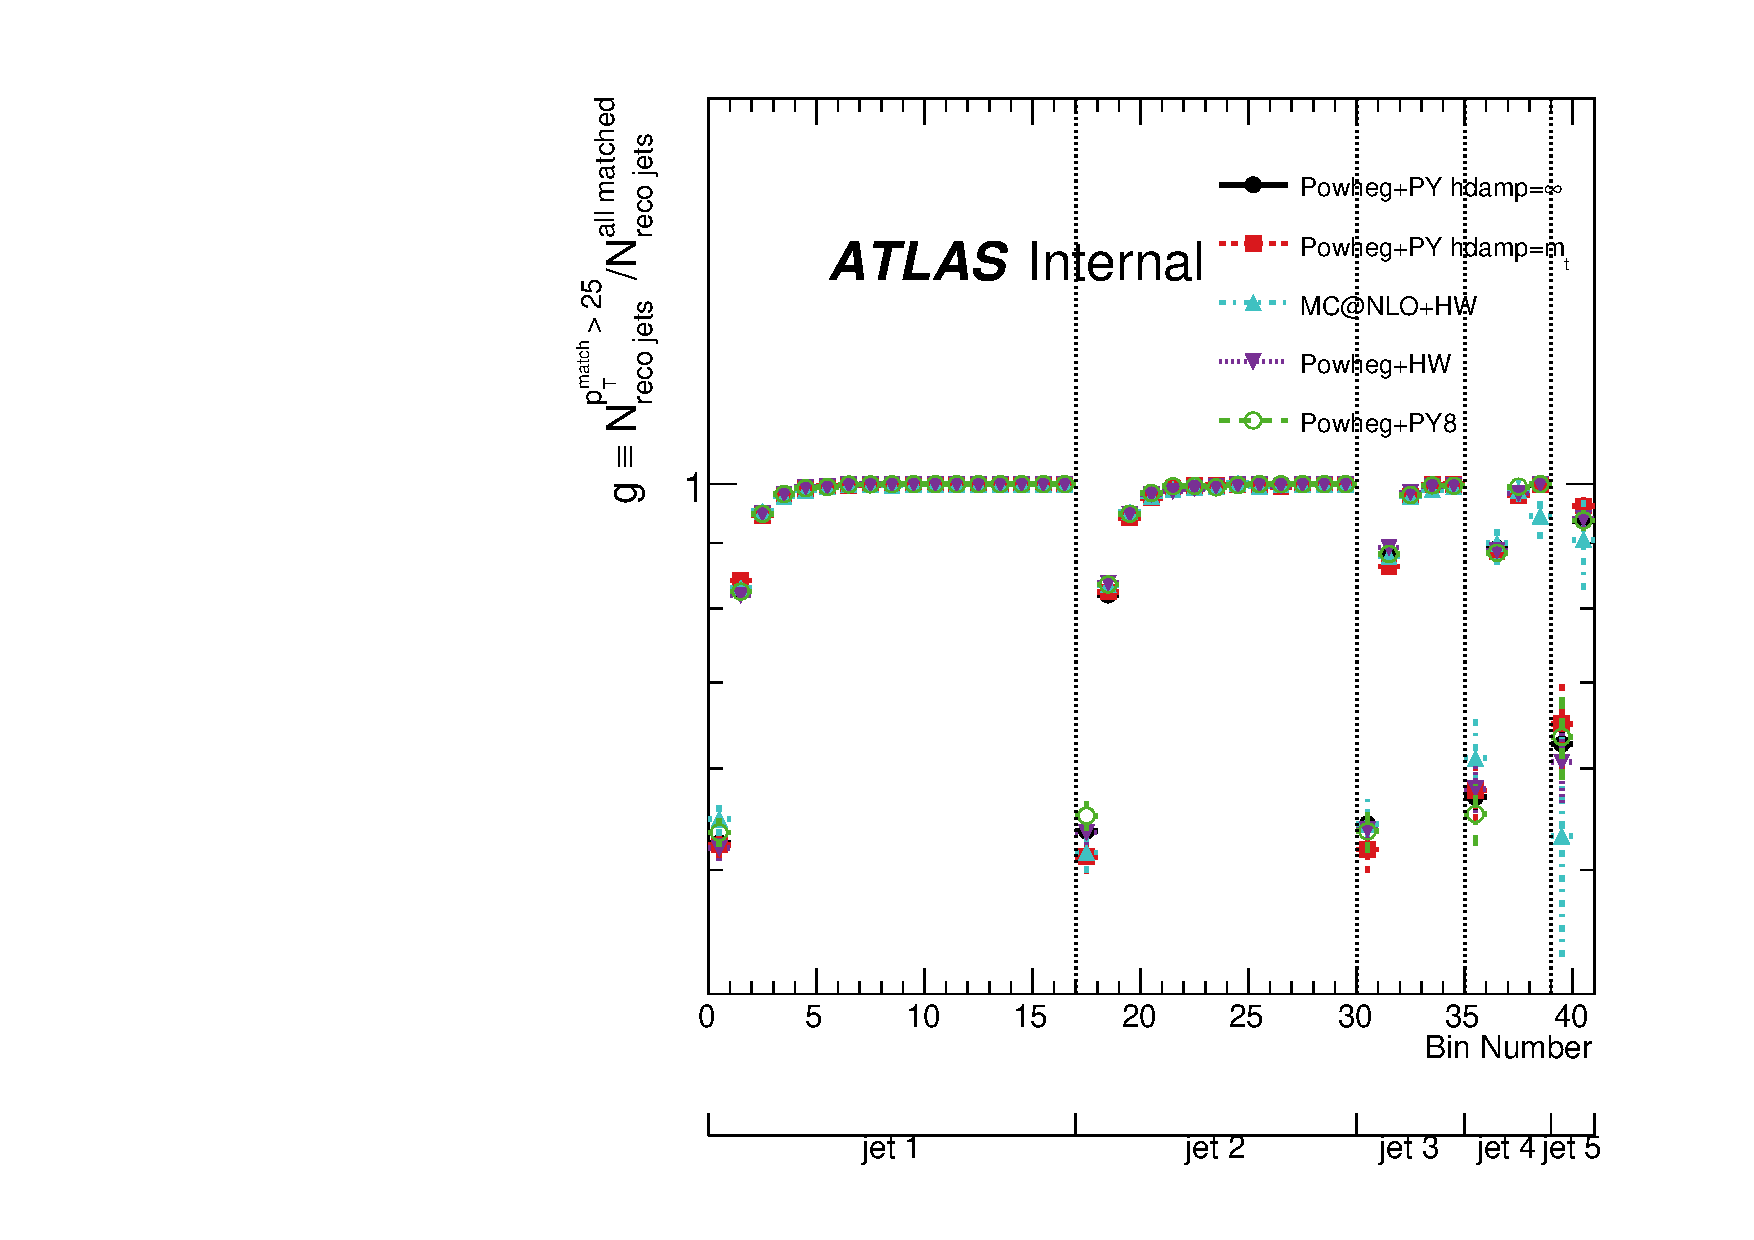
\includegraphics[width=0.45\textwidth]{fig/Unfolding/FeedIn.pdf}
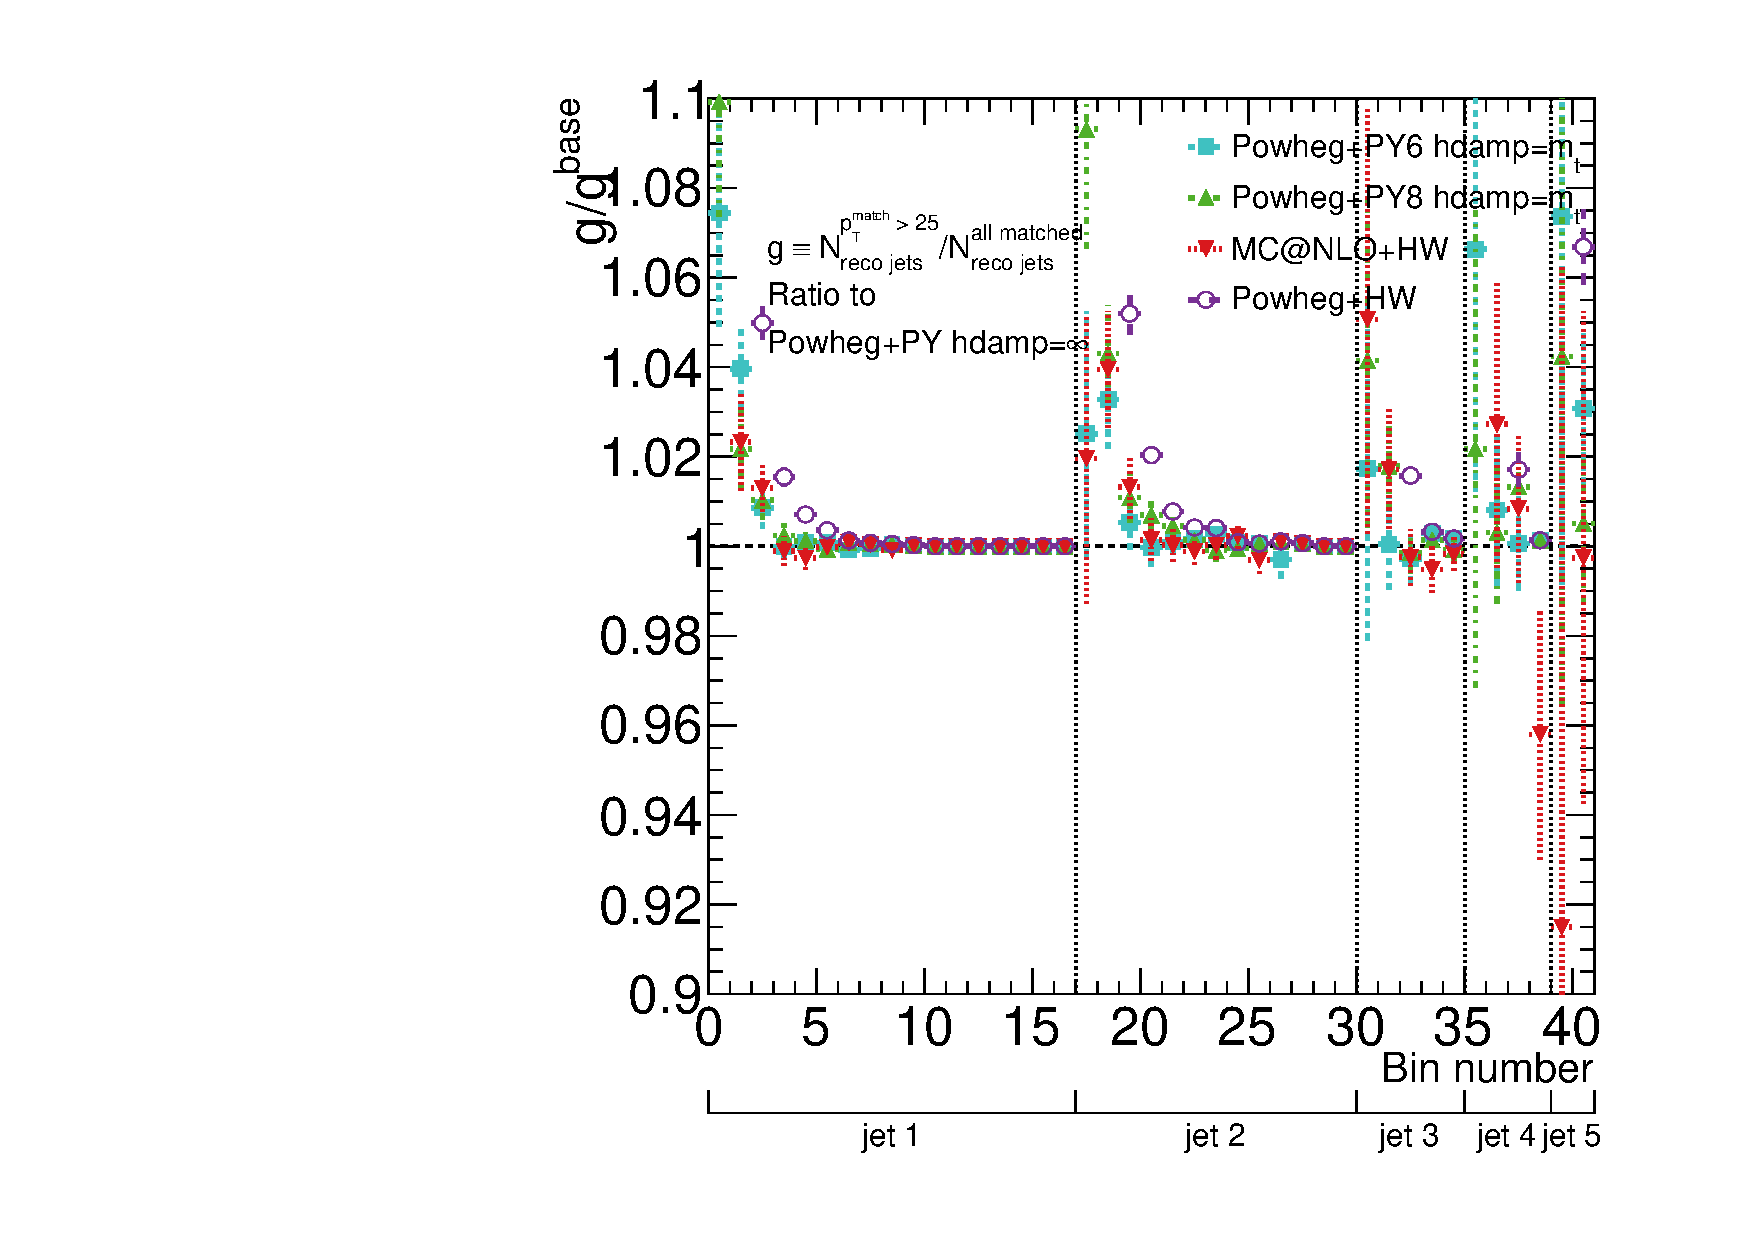
\includegraphics[width=0.45\textwidth]{fig/Unfolding/FeedInFrac.pdf}
\caption{Fraction of reconstructed extra jets with truth matches inside the fiducial region (a) and ratio of alternate generators to the baseline (b). This factor is used to correct the data for \pt\ smearing across the fiducial boundary.}
\label{fig:feedin}
\end{figure}
\subsection{Bias in extra jet distributions due to event selection requirements}
\begin{figure}
\subfloat []{
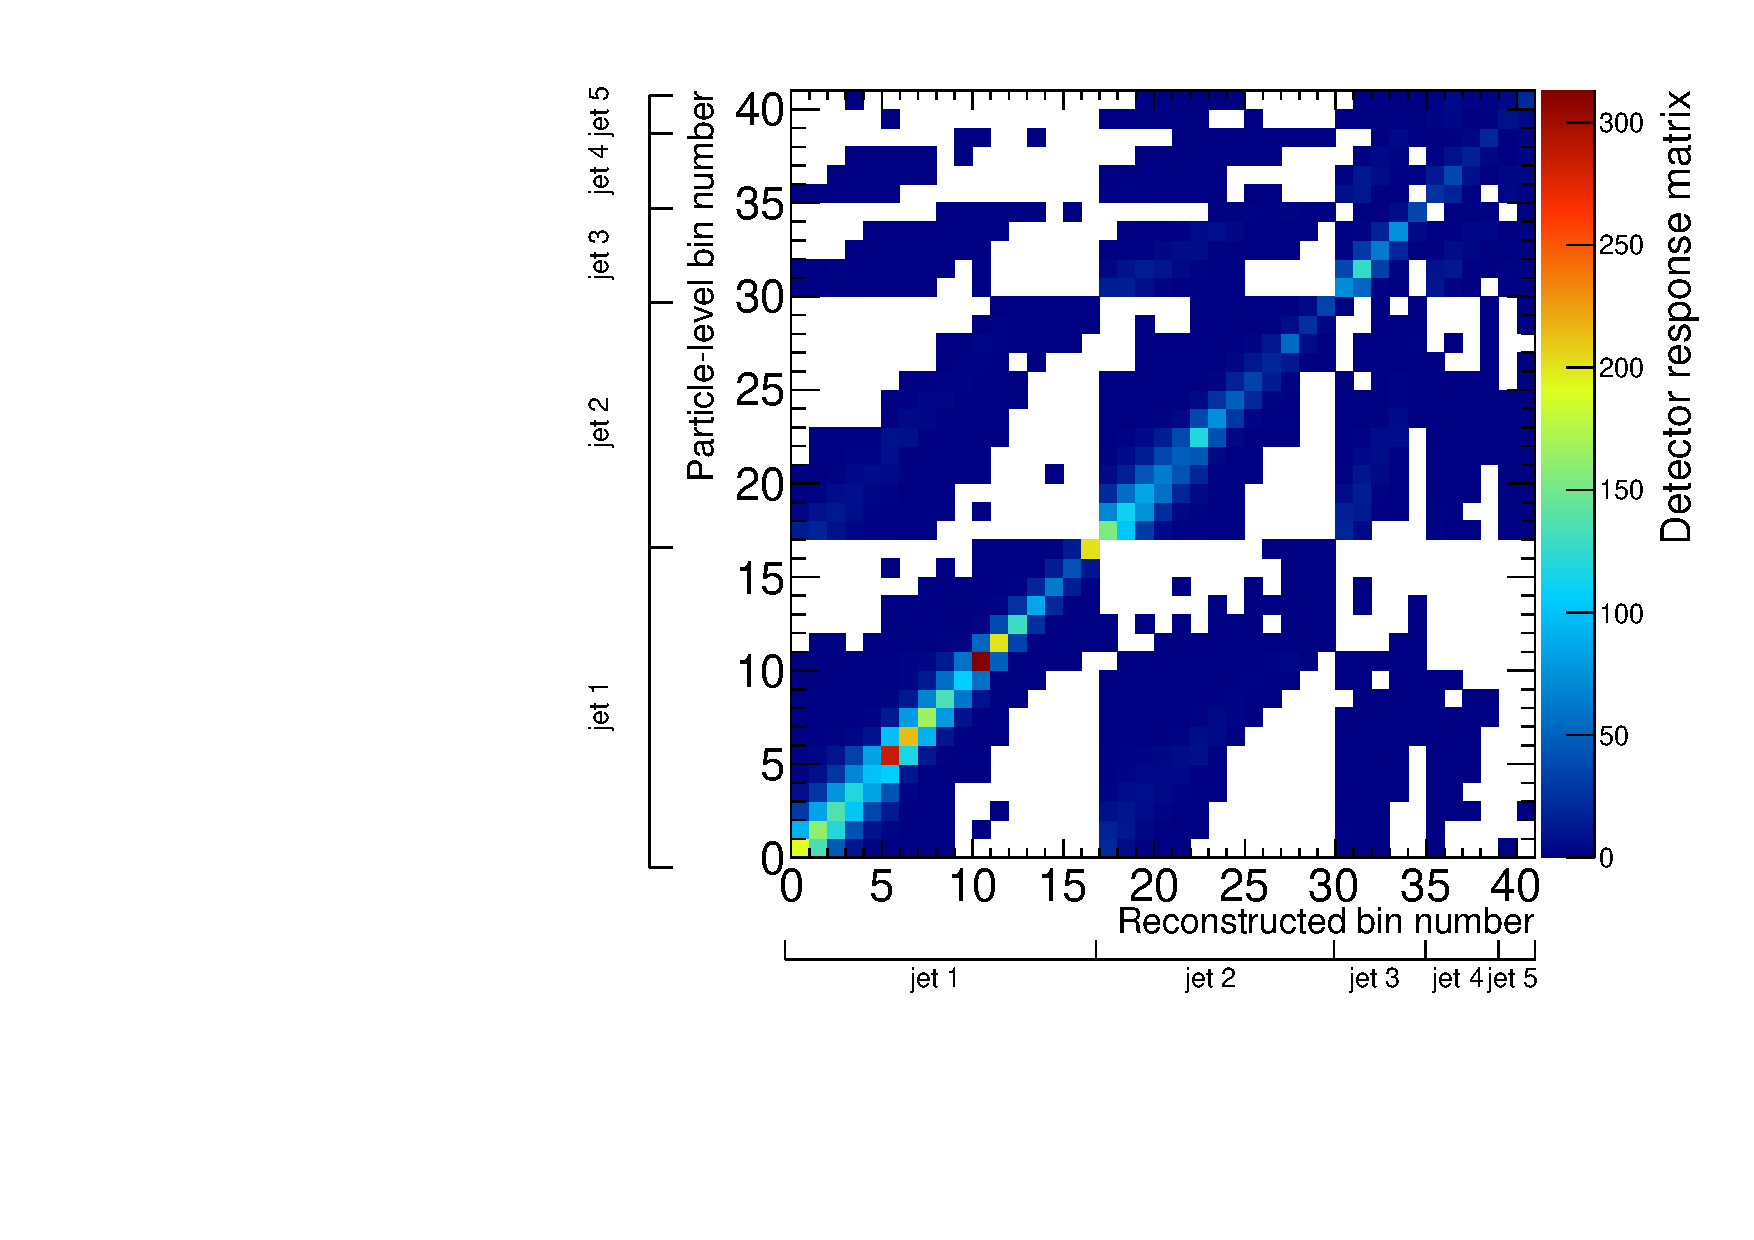
\includegraphics[width=0.45\textwidth]{fig/Cov/Response.pdf}}
~
\subfloat []{
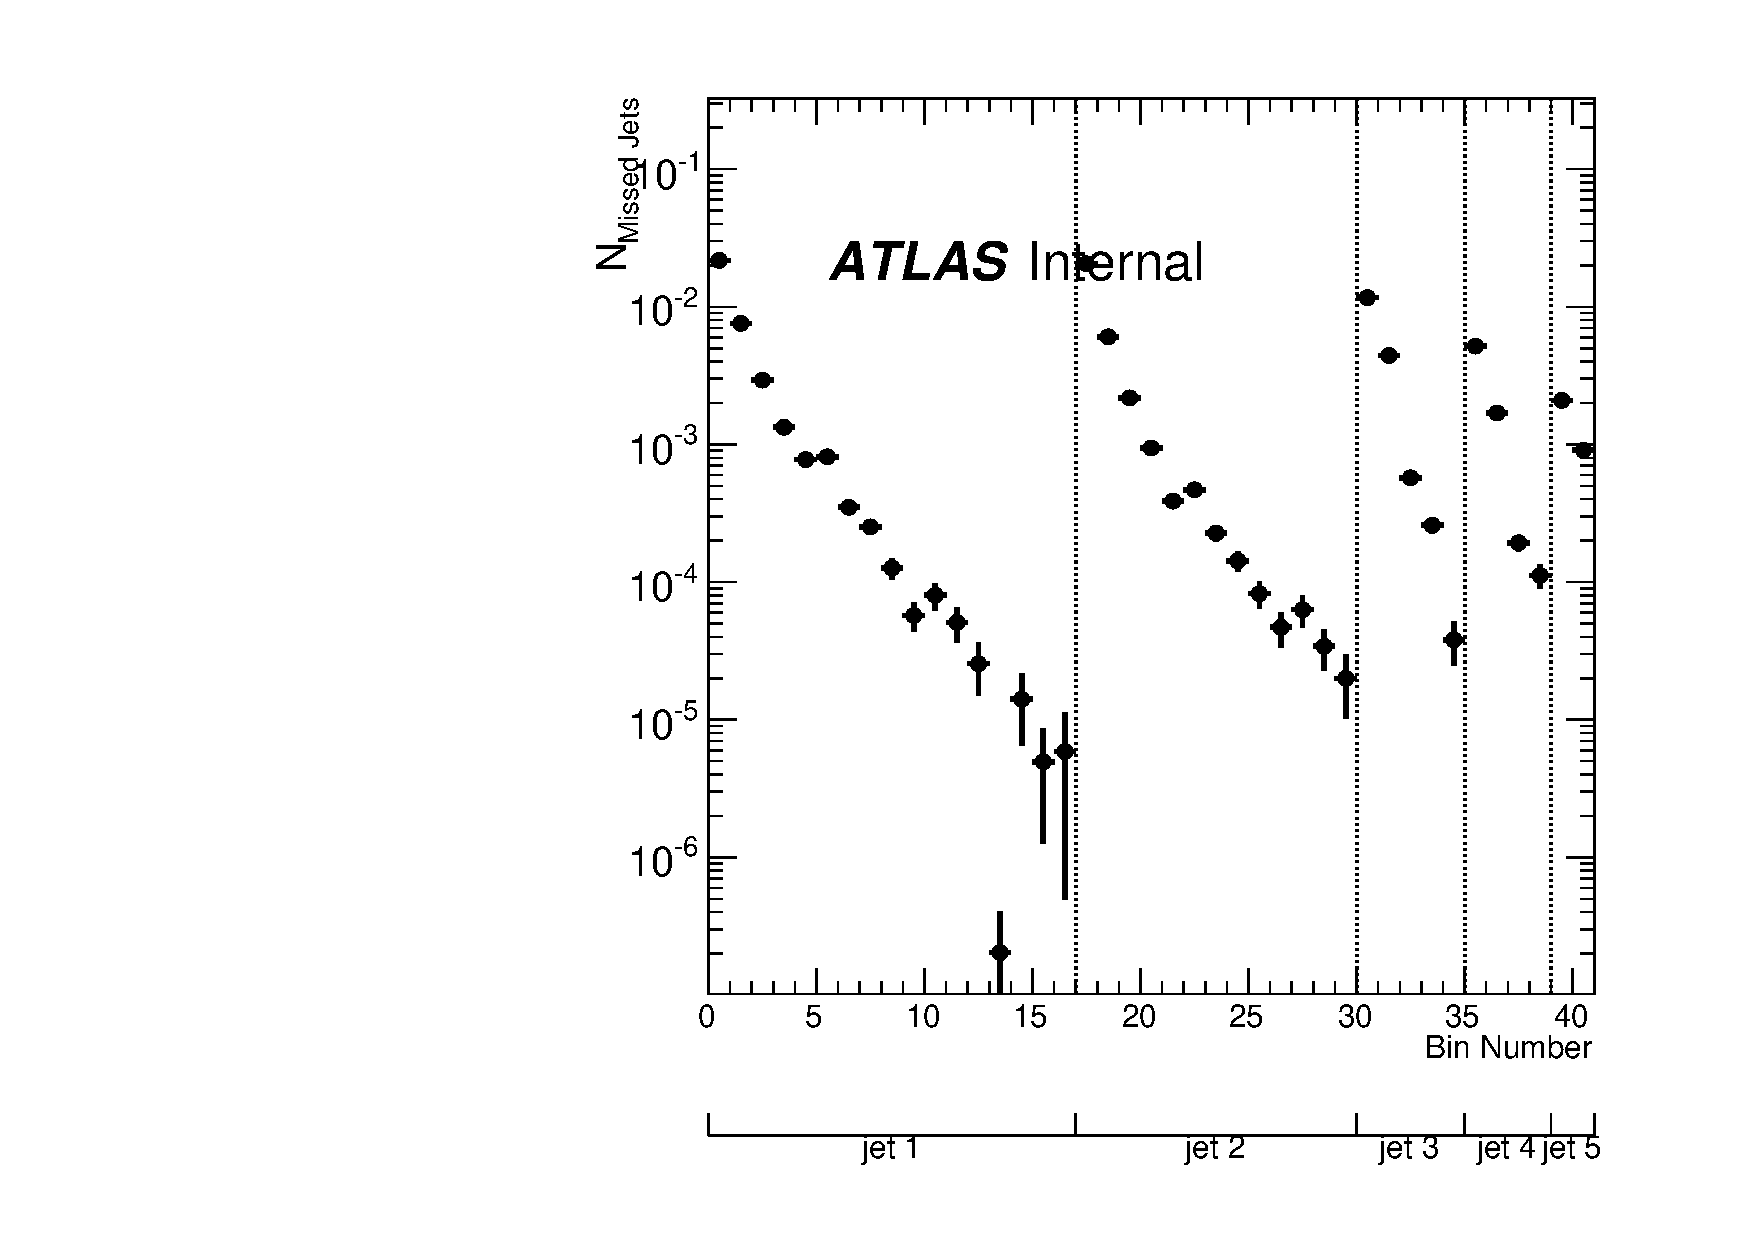
\includegraphics[width=0.45\textwidth]{fig/Cov/MissedPt.pdf}}
~
\caption{Migration matrix between the truth and reconstructed number of extra jets in each bin (a) and distribution of `missed' truth jets not matched to reco jets (b). Jets are binned according to both \pt value and rank. The matrix is filled from events passing both reconstructed and truth $e\mu$+2-$b$ jet events in the baseline \ttbar simulation. `Missed' jets are handled by the RooUnfold framework.}
\label{f:res}
\end{figure}
\label{sec:misid}
% \input{misidentified.tex}

\section{Misidentified events}
The unfolding procedure described above returns unbiased extra jet distributions for
events passing \textit{ both} the truth and reconstruction selection.  This subsample of events has
different kinematics from events passing the truth only selection.  Therefore, the extra jet
distributions obtained from the unfolding are biased with respect to the truth selection.
In addition, a secondary contribution to the bias results from events where one of the two reconstructed
$b$-jets is in fact a mistag.
These biases are corrected using a bin-by-bin correction factor that is applied after the unfolding. 

To understand the contributions to this correction, events that fall outside the combined truth and reconstructed
fiducial region are classified and their kinematic distributions are studied. 
These studies use the~\powpy~\ttbar\ baseline simulation. Table~\ref{t:truthrecoev} gives the number of events passing the fiducial selection for different combinations of reconstruction and truth selection.
Events passing both reconstructed and truth selection are properly handled by the unfolding and used to 
fill the migration matrix, but events that pass one set of selection criteria and not the other 
require additional corrections.  The subsections below provide additional information on each
failure category.

%COMMENT ABOUT MISMATCH OF EXTRA JETS INSIDE TRUTH+RECO EVENT???
\subsubsection{Reconstructed events that fail truth event selection}
Table~\ref{t:reconottruth} shows that $95.85\%$ of reconstructed $e\mu$+2 $b$-jet \ttbar\ events also pass the truth selection
and 4.15\%\ of these are \textit{misclassifed} events that fail. 
This table breaks these events into 5 categories:
%\begin{description}
\begin{enumerate}
\item{Lepton fiducial:} dressed truth $e$ or $\mu$ fails the fiducial $p_{T}$ or $\eta$ cuts, while 
reconstructed $e$ or $\mu$ passes.
\item{Lepton jet overlap:}dressed truth $e$ or $\mu$  overlaps with a truth jet, while reconstructed $e$ or $\mu$ does not overlap with a reconstructed jet.
\item{Lepton non-prompt:} truth $e$ or $\mu$ leptons result from the decay of a hadron or are other background (such as
conversions).
\item{$b$-jet fiducial:} truth $b$-jet fails the fiducial $p_{T}$ or $\eta$ cuts.
\item{$b$-jet other:} truth jet not matched to $B$ hadron, meaning that the reconstructed $b$-jet was mistagged. 
This category also includes a small number of cases where the two reconstructed $b$-jets are matched to a single truth jet or 
one of the two reconstructed $b$-jets does match any truth jet.
\end{enumerate}
%\end{description}
Figure~\ref{fig:reconottruth} shows the electron \pt, $b$-jet \pt, $b$-jet MV1 weight, and extra jet multiplicity 
for events in the above categories. Additional plots of the kinematics and extra jets for these events can be found in Appendix~\ref{app:reconottruth}. 
Events failing the truth lepton or $b$-jet fiducial cuts arise mainly from resolution smearing of the \pt.
These produce a softer spectrum 
%as shown by the peak in the 25-30 \gev\ bin for 
for the reconstructed lepton \pt\ in Figure~\ref{fig:reconottruth}(a) and reconstructed $b$-jet \pt\ in Figure~\ref{fig:reconottruth}(b). 
Misclassified events with overlap between a lepton and a jet show a harder reconstructed lepton \pt\ spectrum and higher extra jet multiplicity, suggesting that a jet has been reconstructed from a lepton. Events with non-prompt leptons show similar properties. 
Finally, in the `$b$-jet other' category, the MV1 of the reconstructed $b$-jet is much lower than other types of events, 
suggesting that a light jet has been mistagged as a $b$-jet. The $\sim 1\%$ rate in this category is consistent with 
the mistag estimate for $b$-jets given in Ref.~\cite{btagmiscal}.

\subsubsection{Truth events that fail reconstructed event selection}
\label{ss:truthNotReco}
Due to detector inefficiencies, the majority of events passing the truth selection fail the reconstruction selection (\textit{missed events}). Table~\ref{t:truthnotreco} shows the events that pass truth selection broken into categories based on which objects were correctly reconstructed. The largest contributions come from failure to reconstruct the electron or the second $b$-jet in the event. A large fraction of these come from migrations across the fiducial boundary due to \pt\ smearing. 

Figure~\ref{fig:truthnotreco} shows the truth $b$-jet \pt, extra jet multiplicity, leading extra jet \pt\ and subleading extra 
jet \pt\ by category. Additional distribtuions can be found in Appendix~\ref{app:truthnotreco}. The $b$-jet \pt\ 
is much softer for events that are not reconstructed. The extra jets in these events are softer as well.

The differences in the extra jet distributions for these events can be explained by studying the relationship between the $b$-jet \pt\ 
and the number and kinematics of the extra jets. Figure~\ref{fig:bjetdep} shows the extra jet multiplicity and \pt\ in truth events in 
bins of $b$-jet \pt. Softer $b$-jets correspond to events with softer and fewer extra jets. This effect is likely the result of 
the dependence of the  $b$-jet \pt\ on \pttop. 

In summary, events that fail the reconstruction requirements on the $b$-jets have a lower extra jet multiplicity and 
softer jets than those that fall in other categories.   
%Although the extra jets in events that fail reconstruction differ significantly from those that pass, the difference can be understoood as a bias in \pttop. (TODO??) A systematic uncertainty on this difference can be set by varying \pttop .



\begin{table}
\begin{center}
\begin{tabular}{|l|c|}
\hline
Category & $N_{\textrm{events}}$\\
\hline
Reco & 11997.1 \\
Truth & 43496.9 \\
Reco AND truth & 11499.0 \\
Reco AND NOT truth & 498.2 \\
NOT Reco AND truth & 31877.7 \\
\hline
\end{tabular}
\end{center}
\caption{Number of events passing different combinations of truth and reconstructed selection requirements.}
\label{t:truthrecoev}
\end{table}

\begin{table}
\begin{center}
\begin{tabular}{|l|cc|}
\hline
Category & $N_{\textrm{events}}$ & (\%) \\
\hline
Lepton fiducial & 67.5 & 0.56 \\
Lepton jet overlap & 50.6 & 0.42 \\
Lepton non-prompt & 10.9 & 0.09 \\
$b$-jet fiducial & 245.8 & 2.05 \\
$b$-jet other & 123.4 & 1.03 \\
\hline
Total misclassified & 498.2 & 4.15 \\
\hline \hline
Passes reco and truth selection & 11499.0 & 95.85 \\
\hline
Total reco events & 11997.1 & 100.00 \\
\hline
\end{tabular}
\end{center}
\caption{Number of selected reconstructed events that fail truth selection categorized by reason they have failed.  The selections are applied sequentially in the order listed in the table.}
\label{t:reconottruth}
\end{table}

\begin{figure}
\centering
\subfloat{
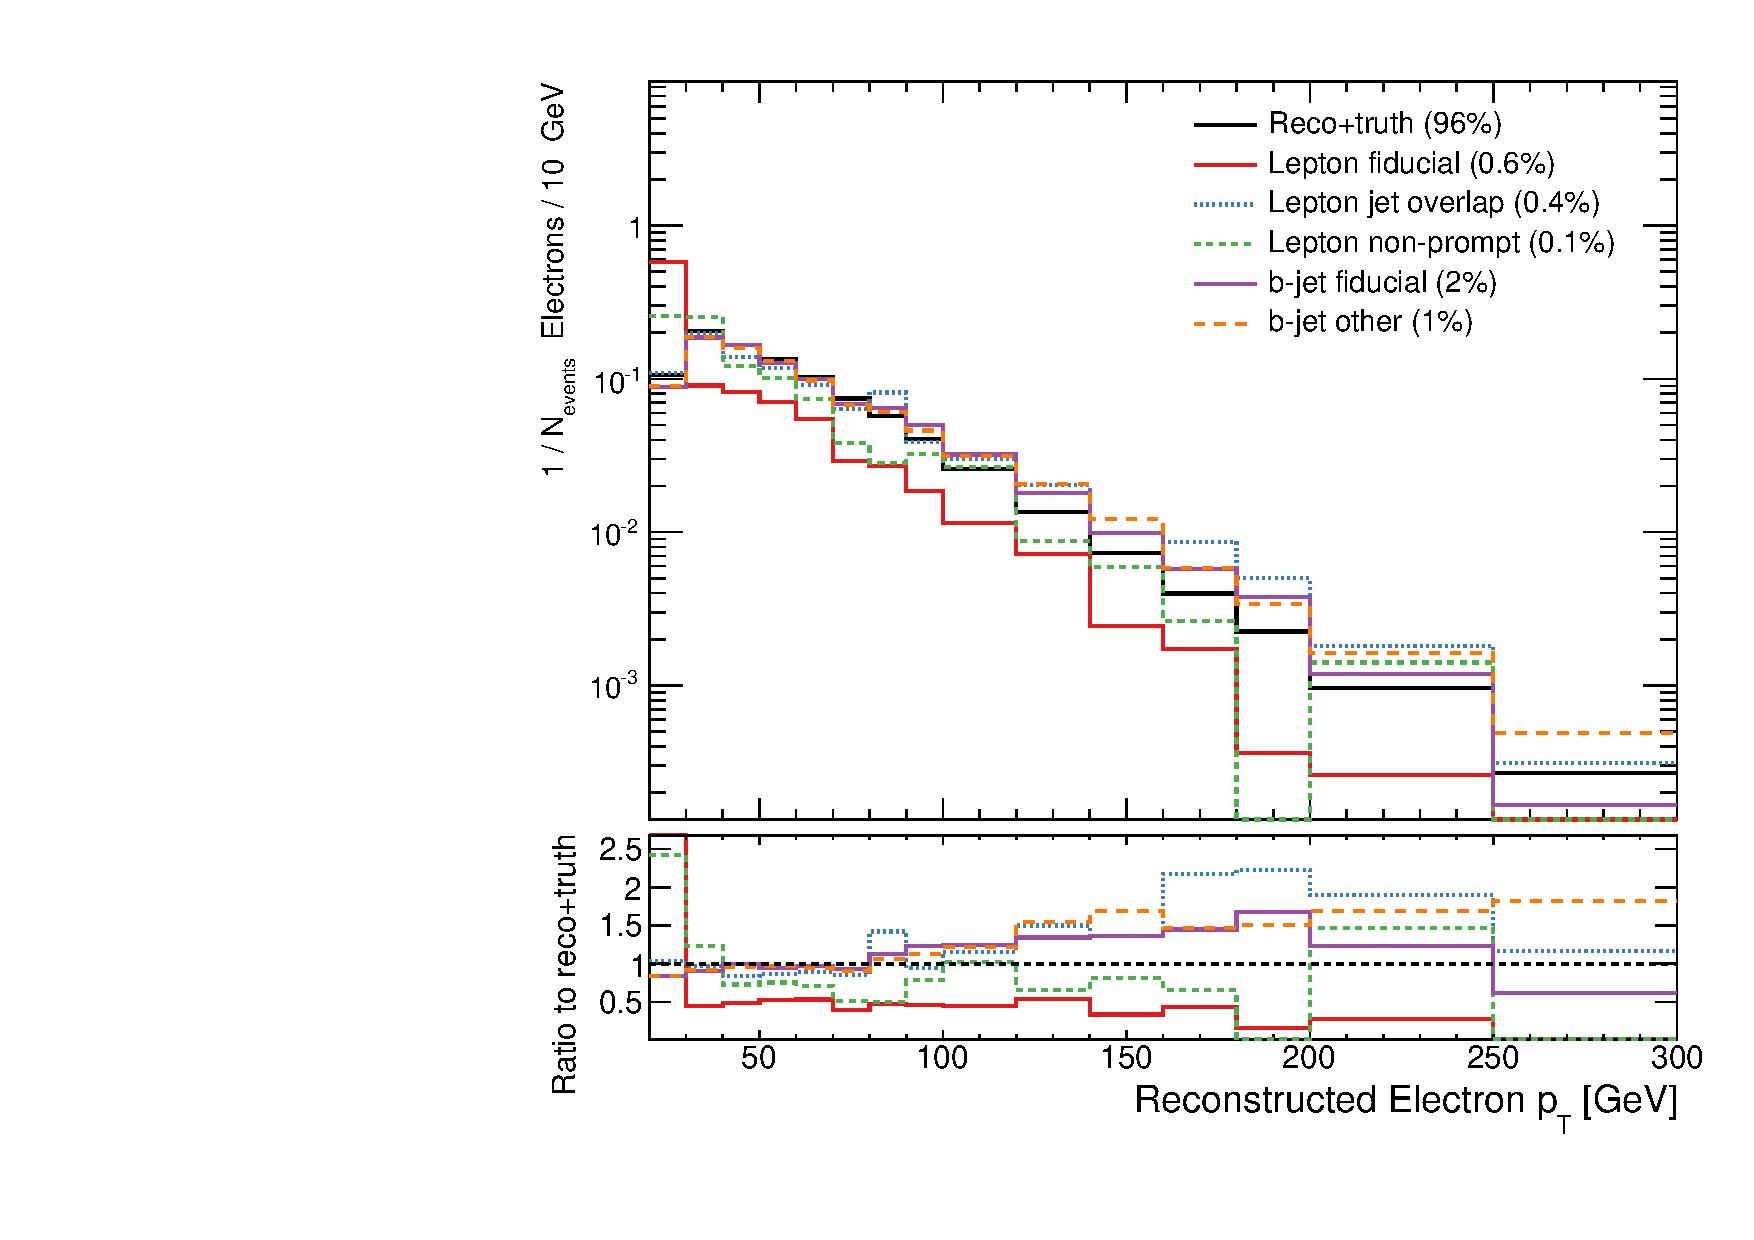
\includegraphics[width=0.45\textwidth]{fig/RecoNotTruth/ElecPt.pdf}}
\subfloat{
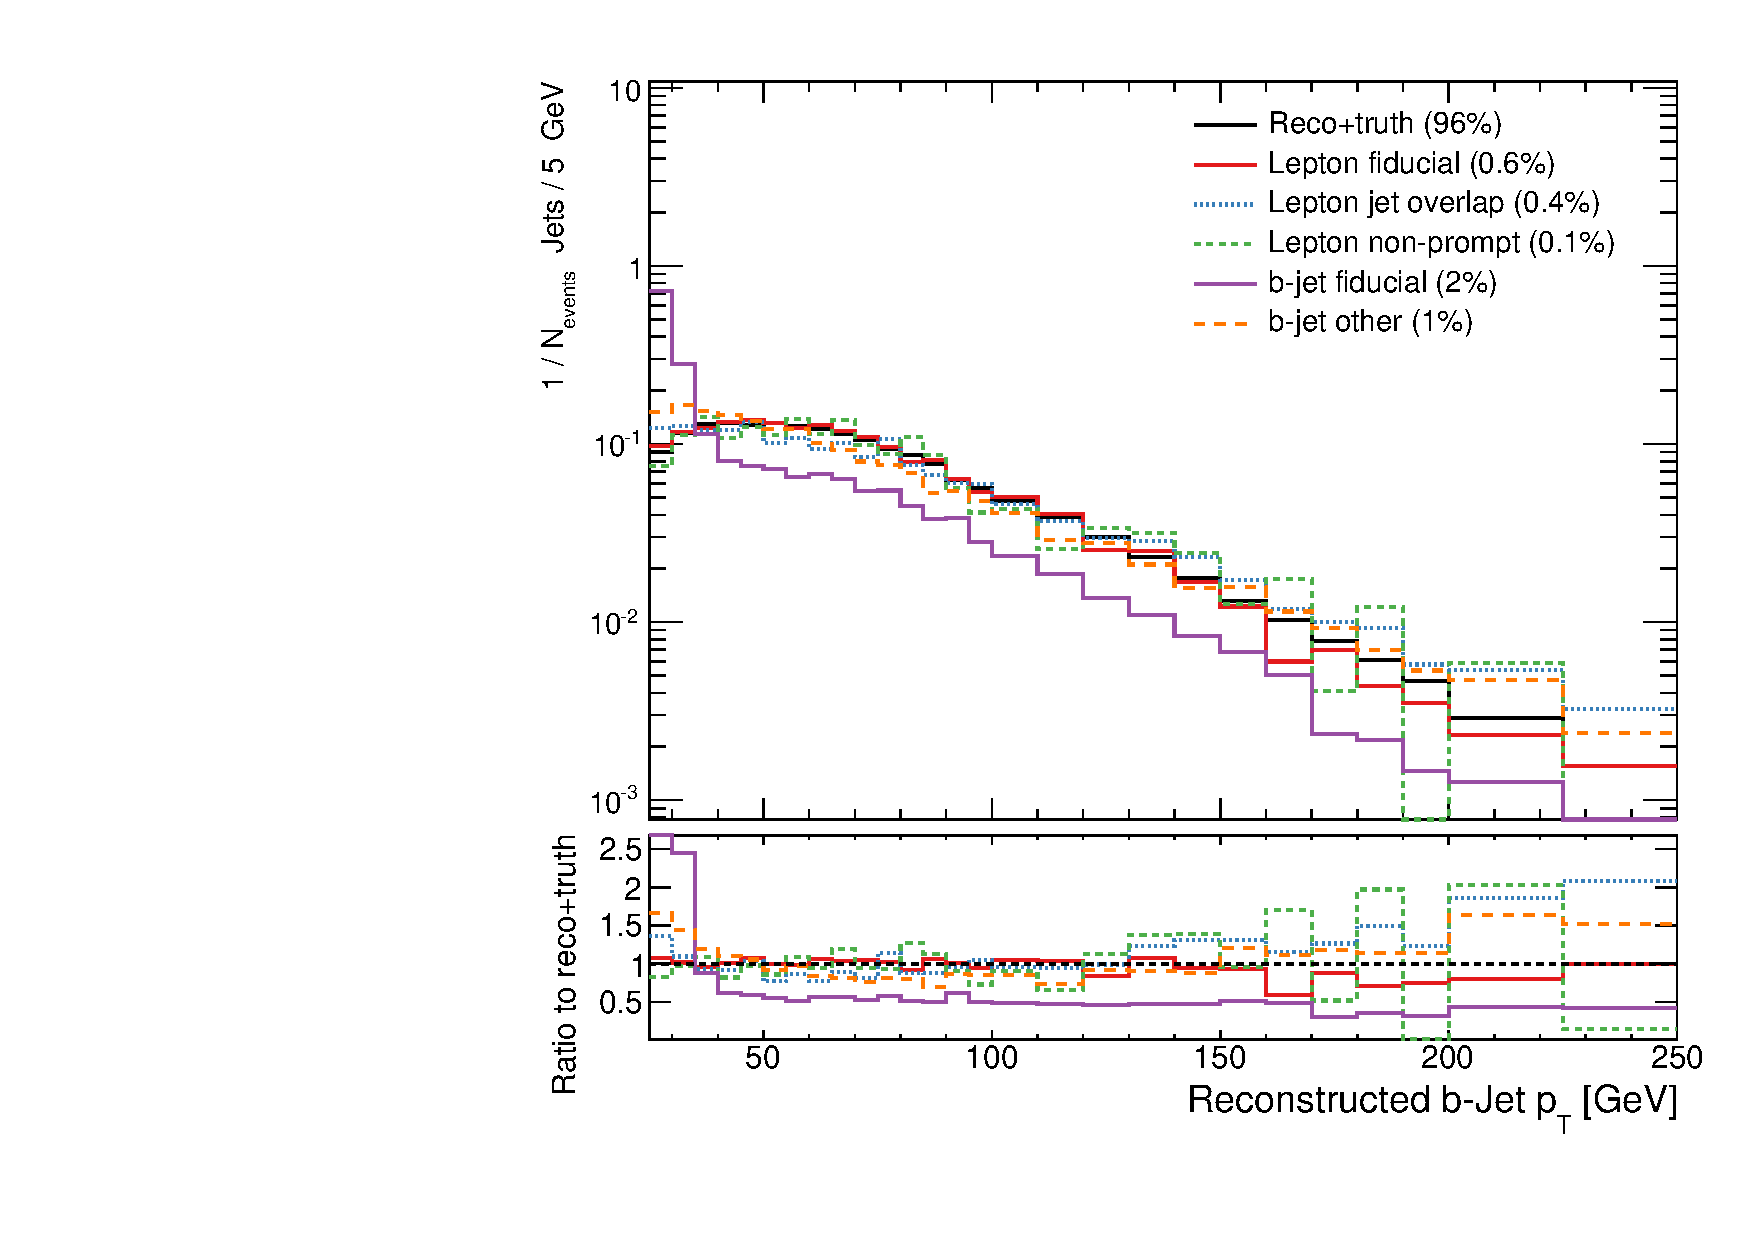
\includegraphics[width=0.45\textwidth]{fig/RecoNotTruth/BJetPt.pdf}}
\\
\subfloat{
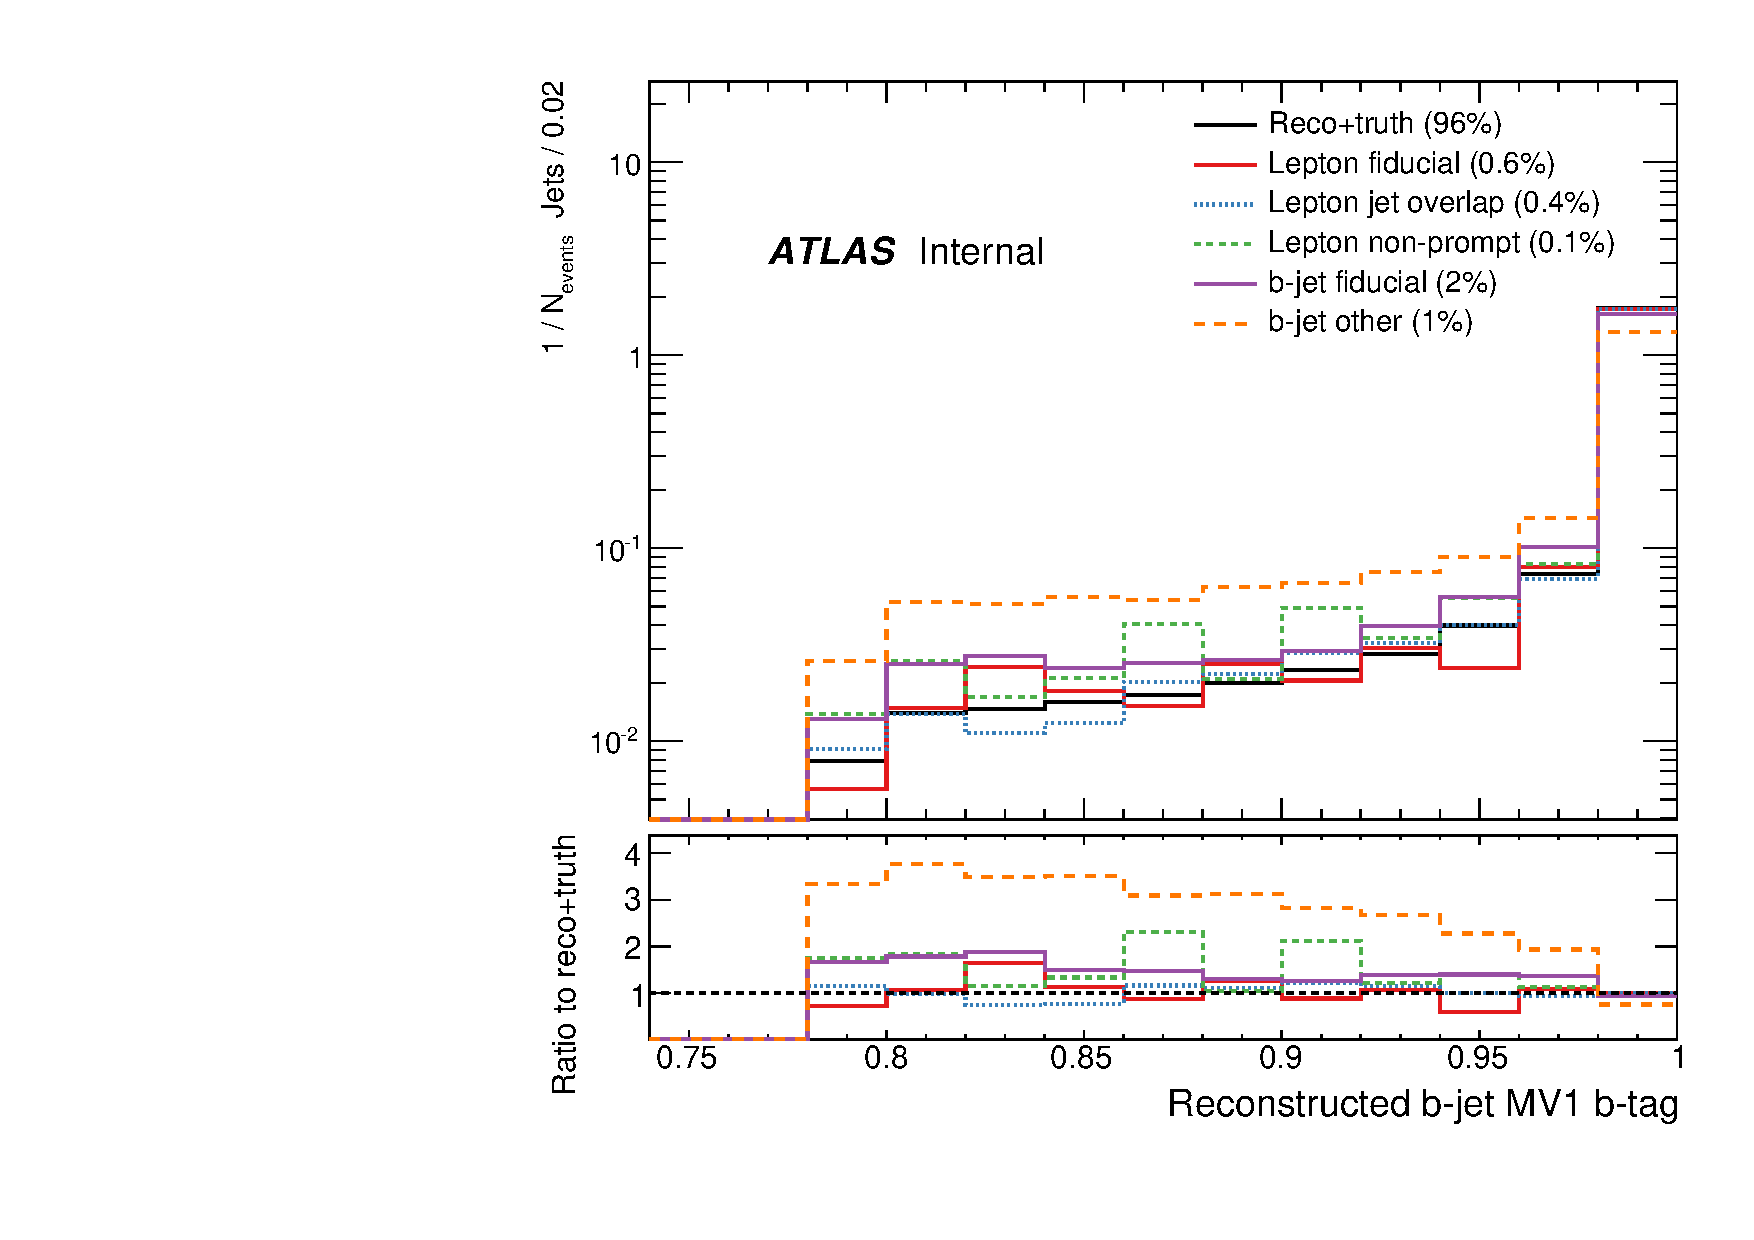
\includegraphics[width=0.45\textwidth]{fig/RecoNotTruth/BJetMV1.pdf}}
\subfloat{
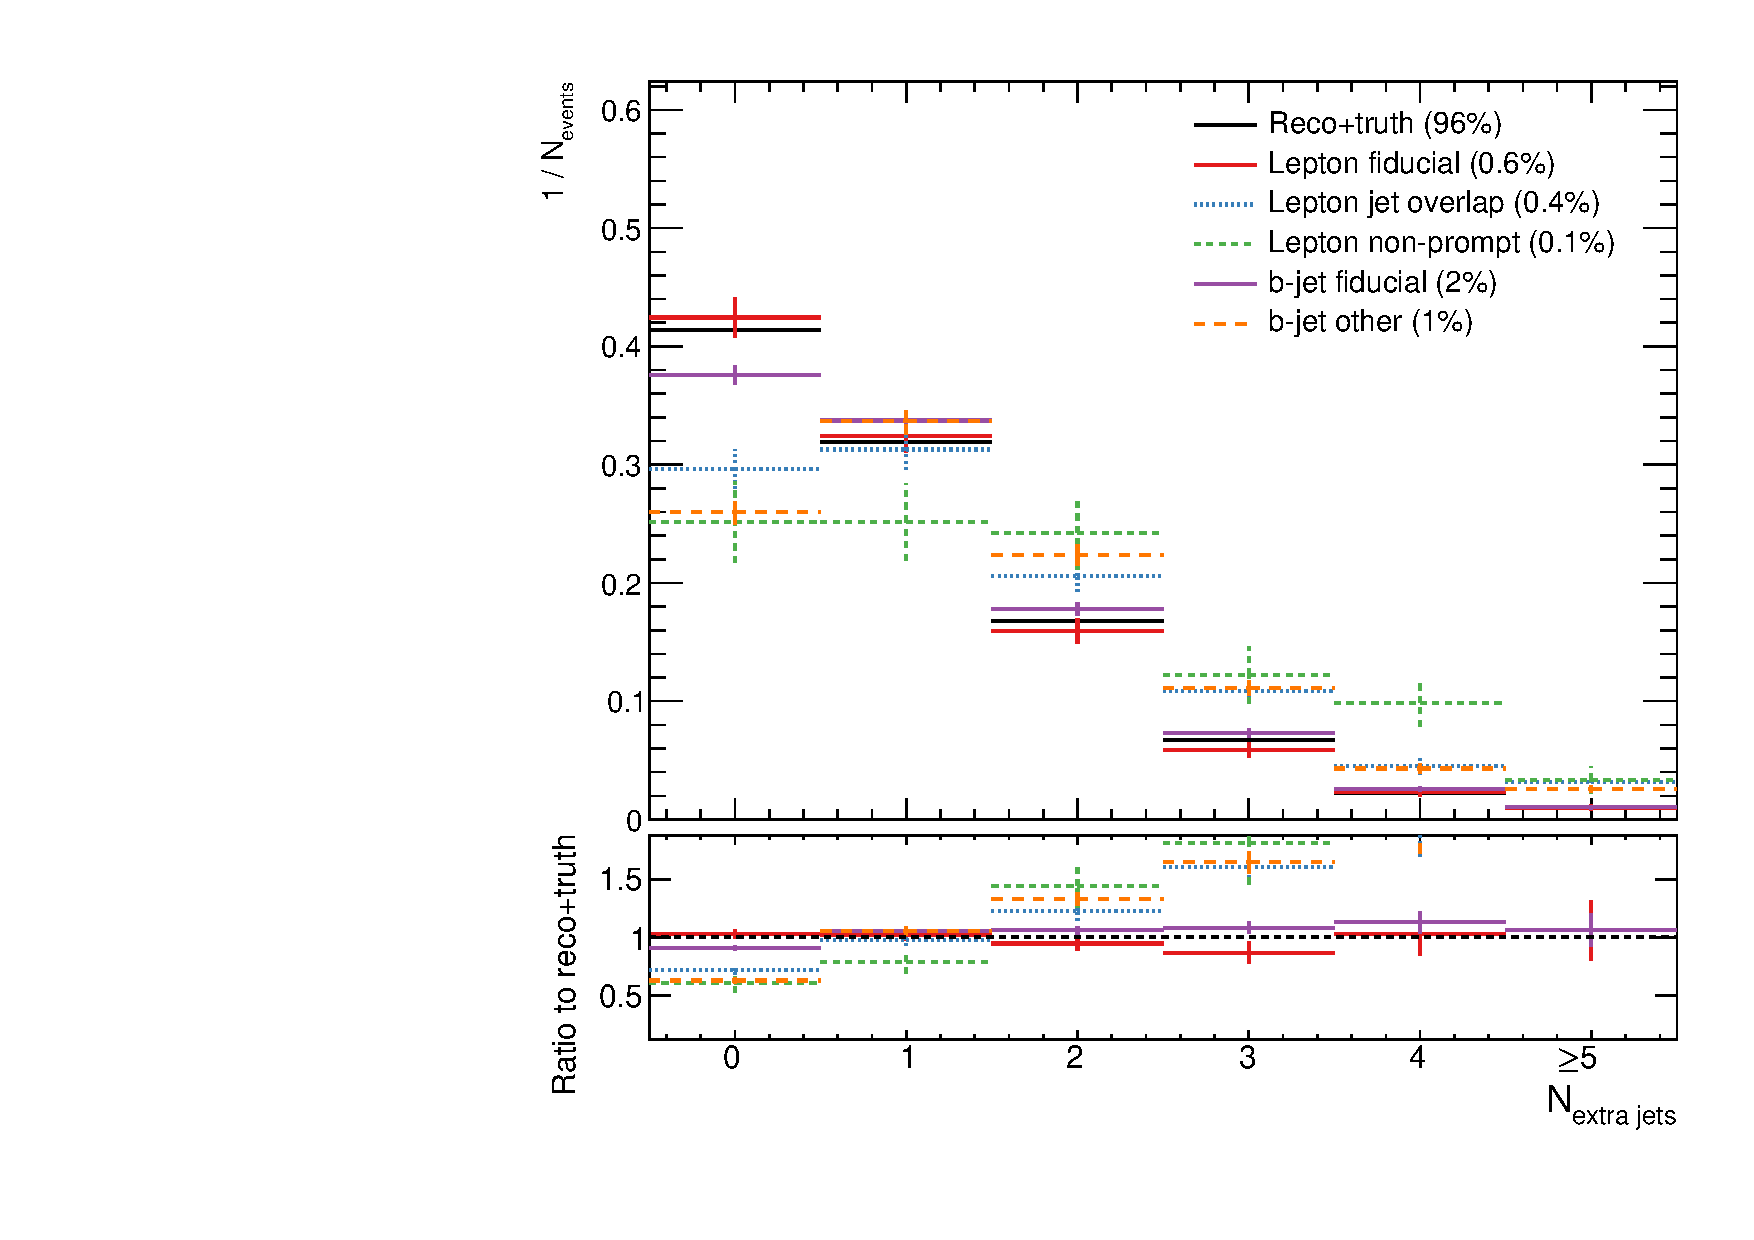
\includegraphics[width=0.45\textwidth]{fig/RecoNotTruth/NJets.pdf}}
\caption{Distributions of the (a) $e$ \pt, (b) $b$-jet \pt, (c) $b$-jet MV1 weight and (d) extra jet multiplicity. Each distribution is normalized by the number of events falling in that category. Events were simulated with \powpy~\ttbar.}
\label{fig:reconottruth}
\end{figure}


\begin{table}
\begin{center}
\begin{tabular}{|l|cc|}
\hline
Category & $N_{\textrm{events}}$ & (\%) \\
\hline
No $e$ & 13472.3 &	31.06 \\
No $\mu$ & 3743.0 & 8.63 \\
same-sign $e\mu$ & 161.1 & 0.37 \\
0 $b$-jets & 2986.0	& 6.88 \\
1 $b$-jet  & 11515.3 & 26.55 \\
\hline
Missed total & 31877.7 & 73.49 \\
\hline \hline
Passes reco and truth selection & 11499.0 & 26.51 \\
\hline
Total truth events & 43376.7 & 100.00 \\
\hline

\end{tabular}
\caption{Number of truth events that fail reconstruction selection categorized by reason they have failed. The selections are applied sequentially in the order listed in the table.}
\label{t:truthnotreco}
\end{center}
\end{table}

\begin{figure}
\centering
\subfloat{
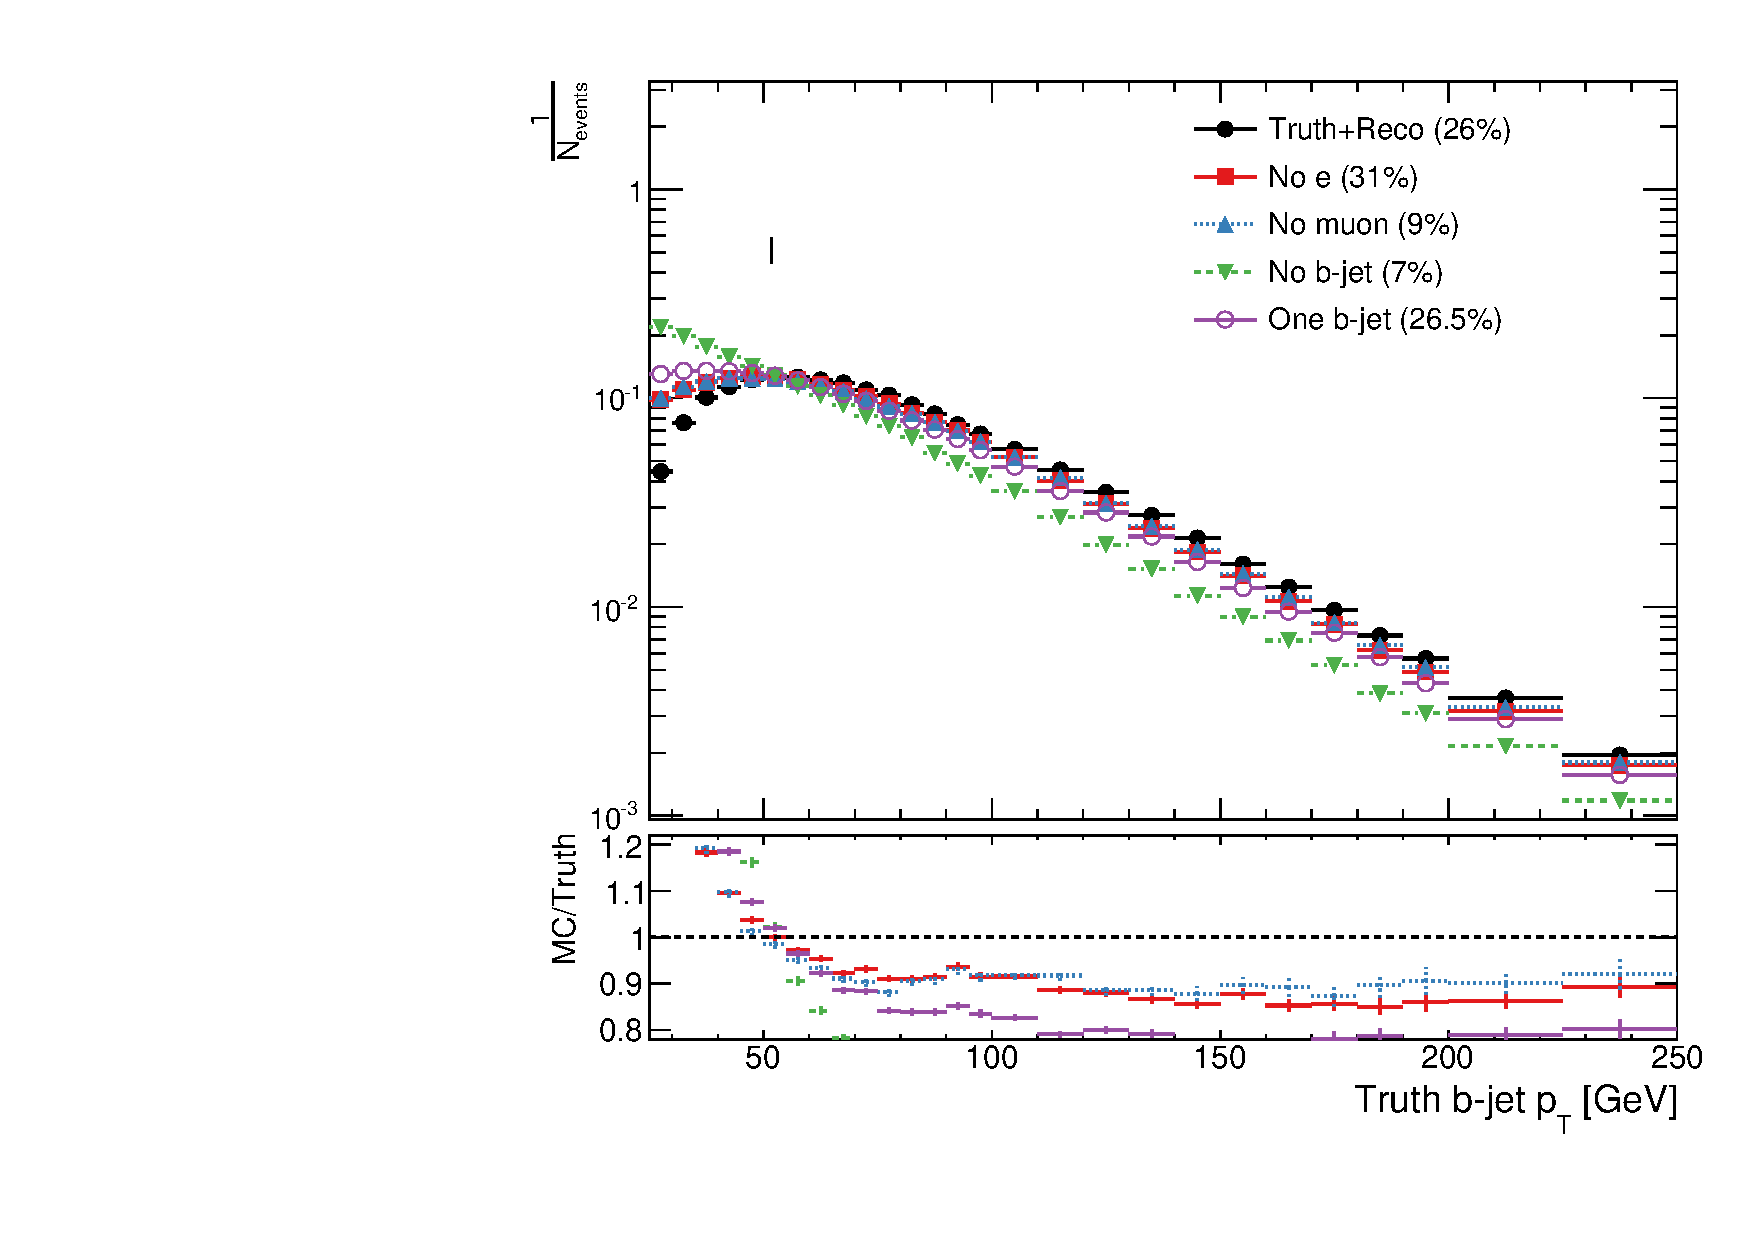
\includegraphics[width=0.45\textwidth]{fig/TruthNotReco/TruthBJetPt.pdf}}
\subfloat{
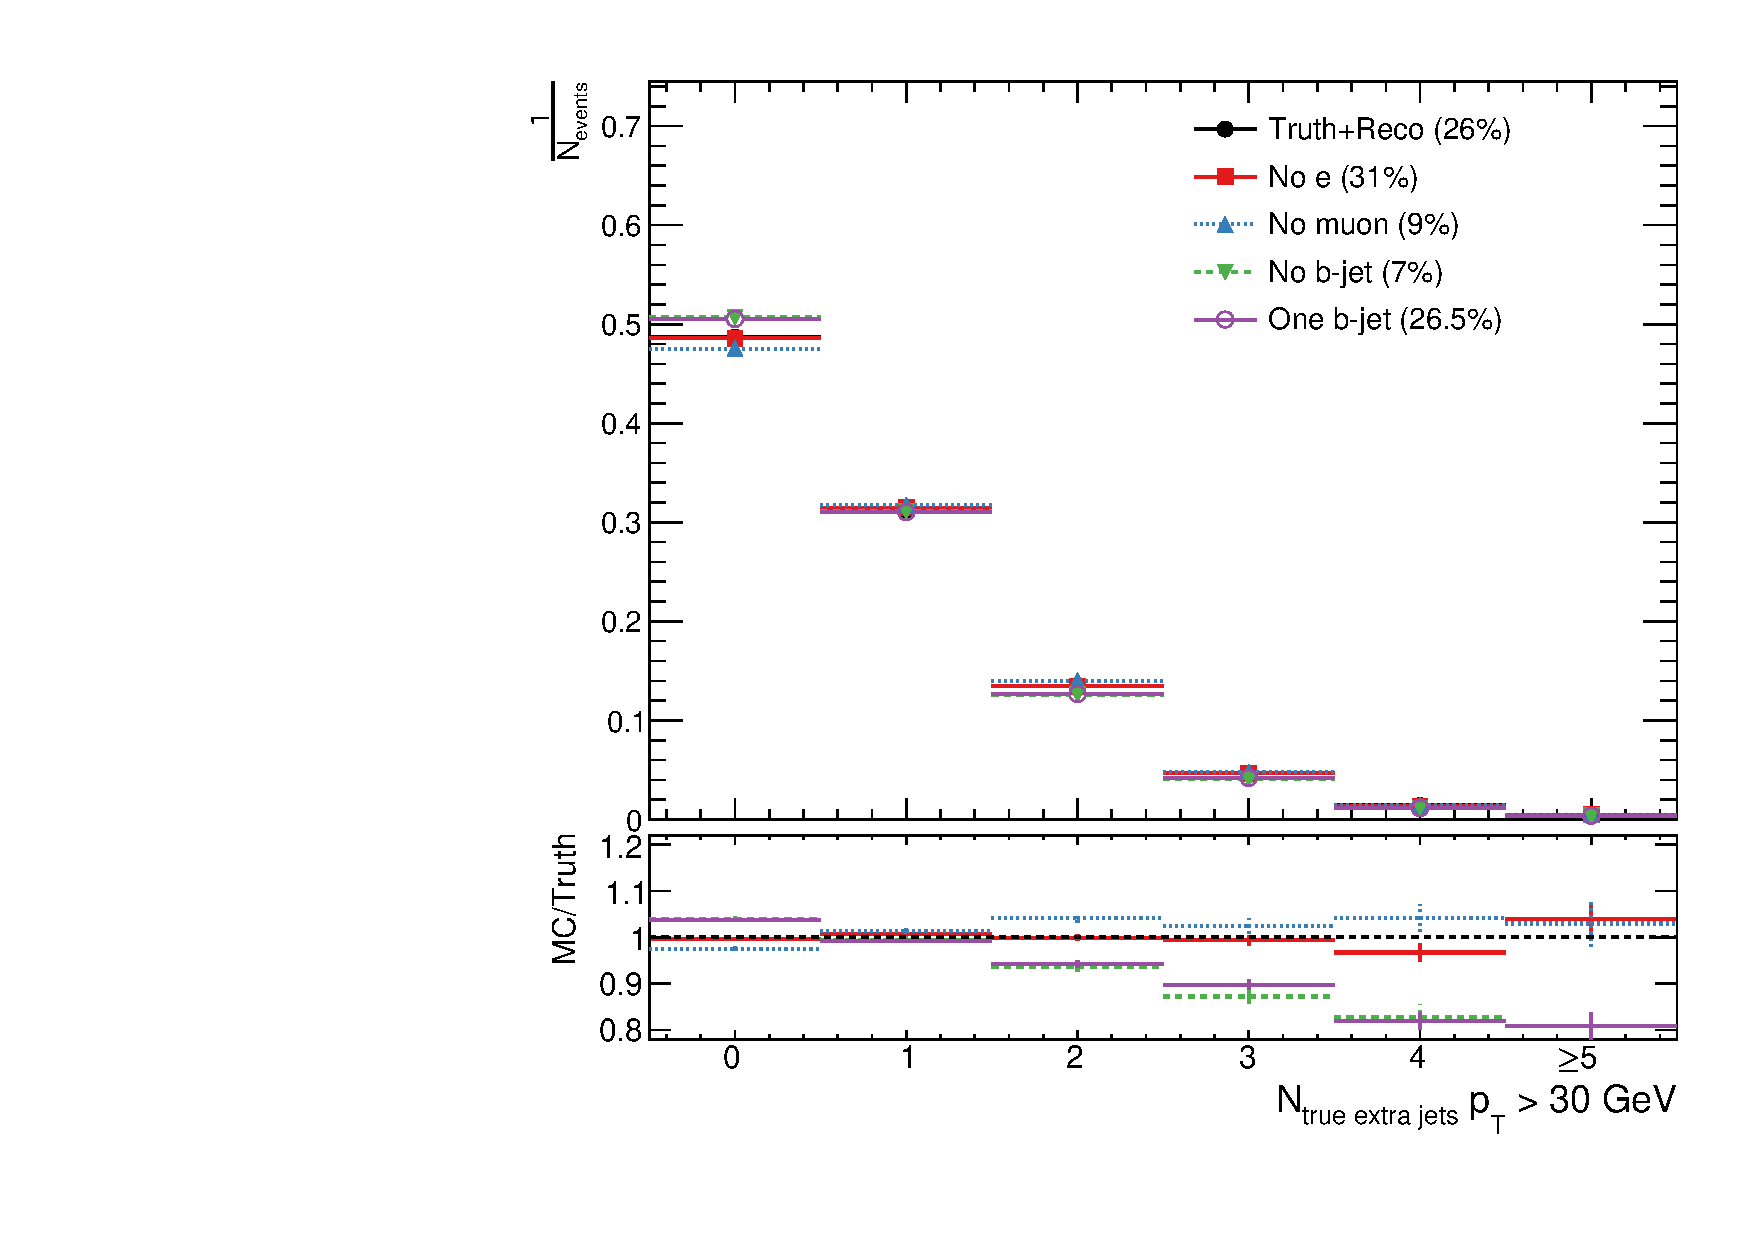
\includegraphics[width=0.45\textwidth]{fig/TruthNotReco/NTruthExtraJets30.pdf}}
\\
\subfloat{
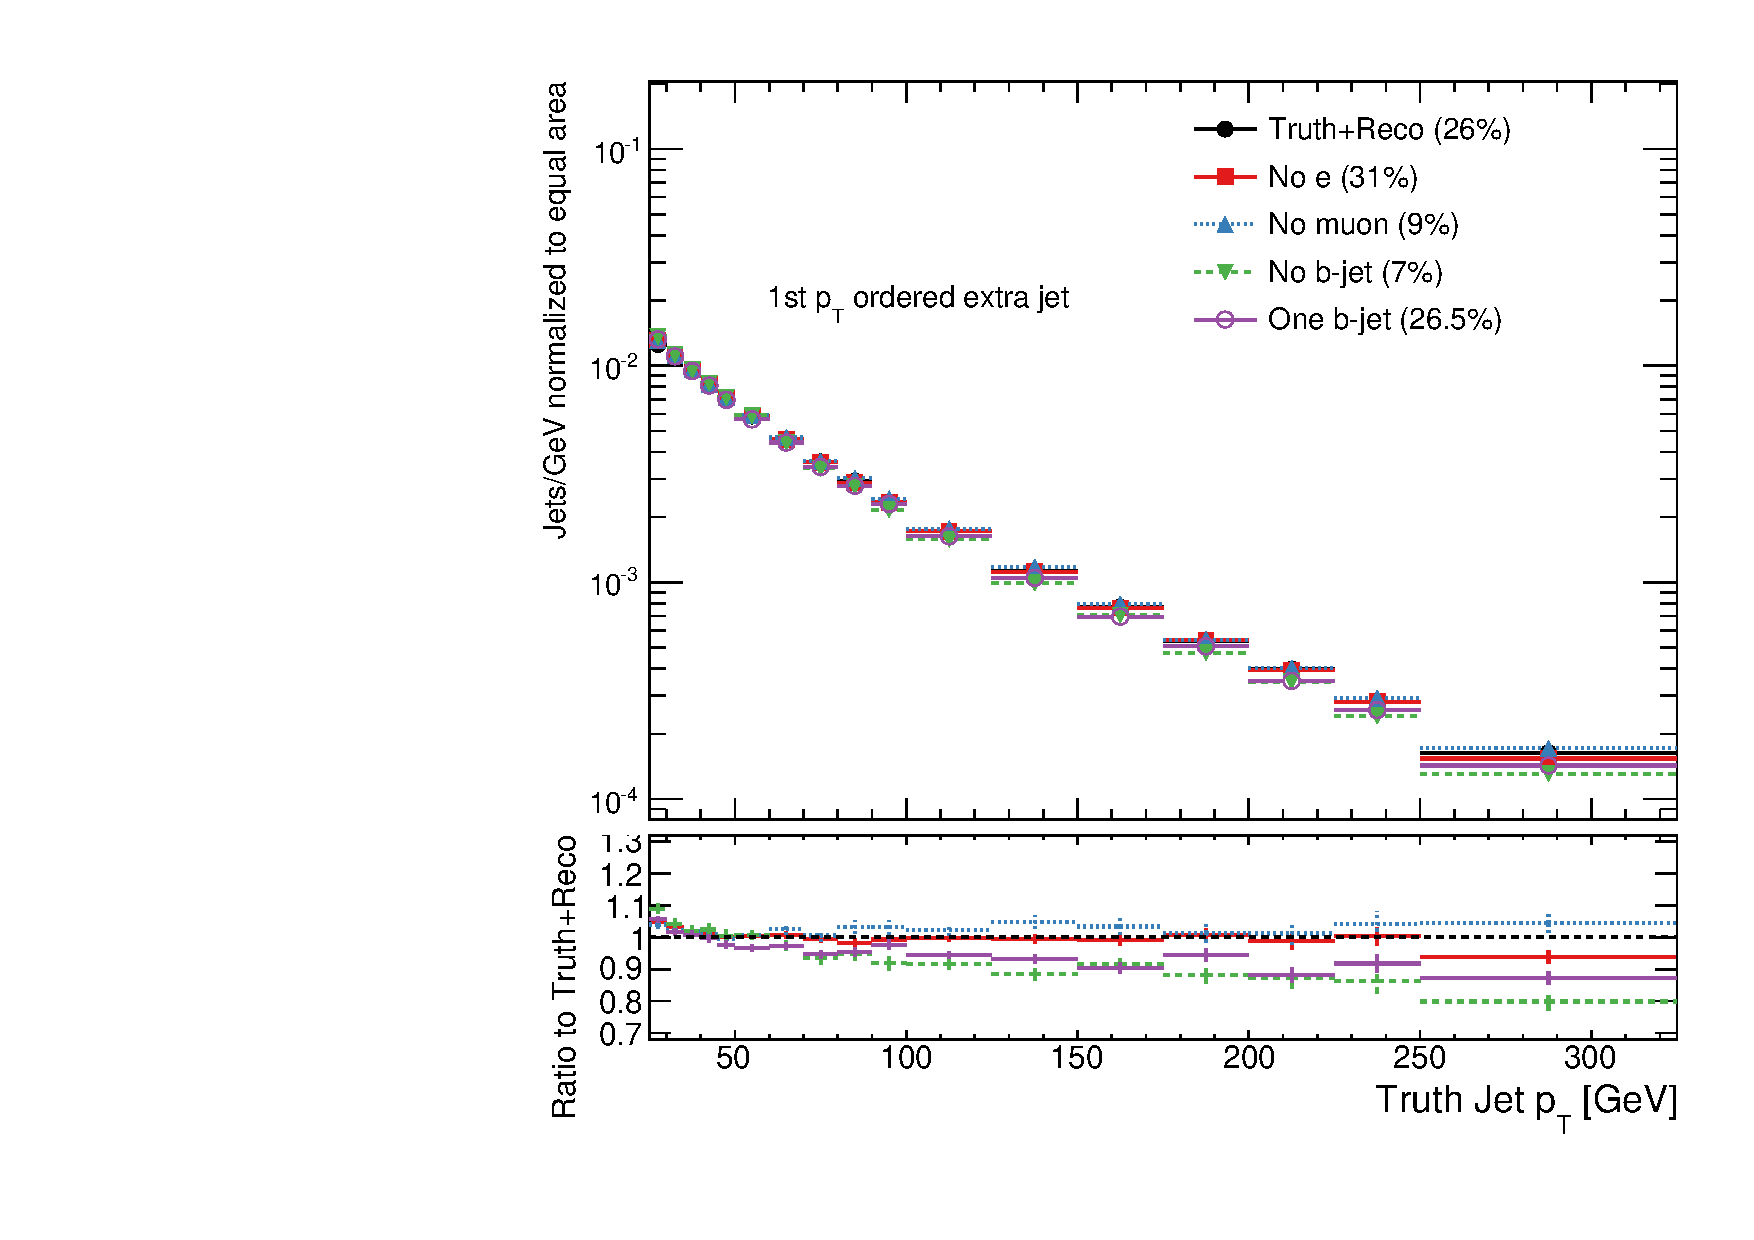
\includegraphics[width=0.45\textwidth]{fig/TruthNotReco/TruthPtJet0.pdf}}
\subfloat{
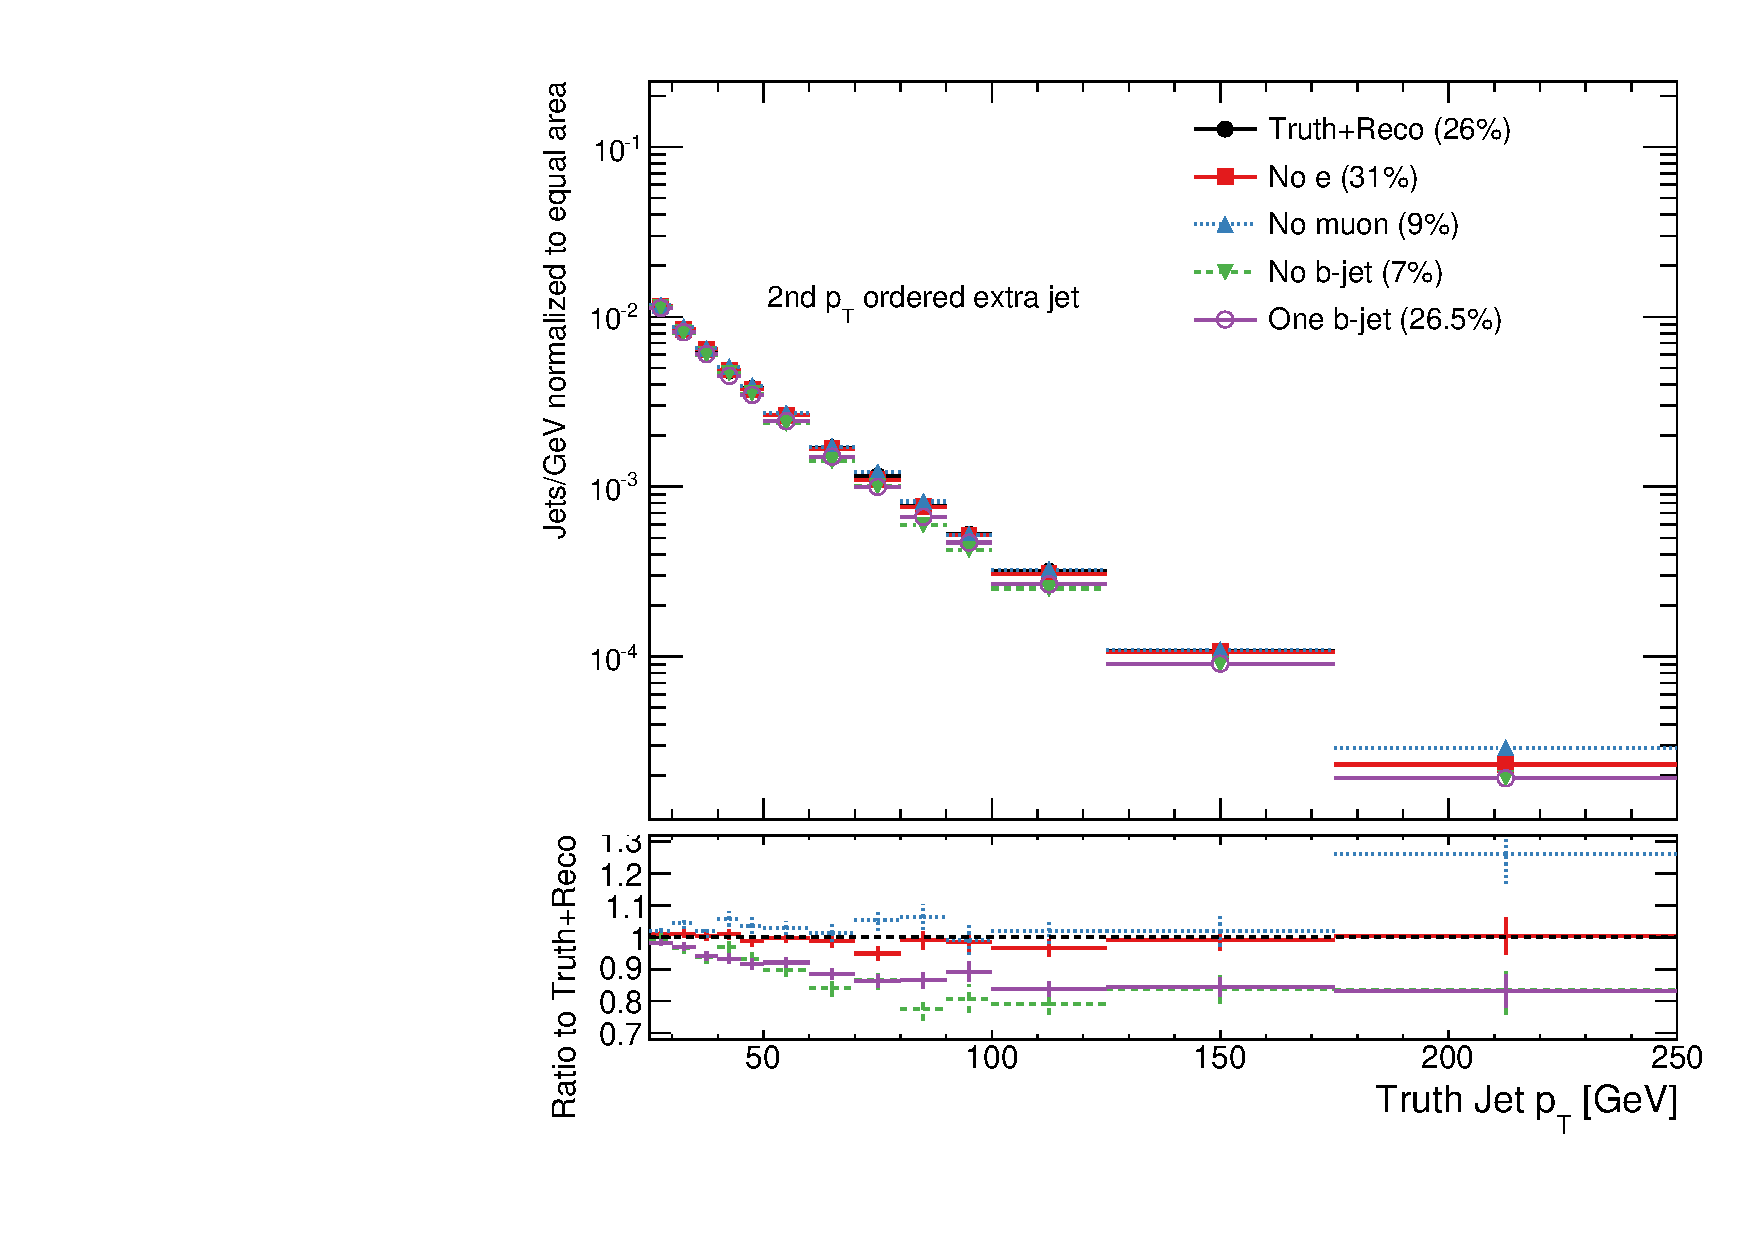
\includegraphics[width=0.45\textwidth]{fig/TruthNotReco/TruthPtJet1.pdf}}
\caption{Distributions of the truth (a) $b-$jet \pt, (b) extra jet multiplicity, (c) leading extra jet \pt and (d) subleading extra jet \pt. Each distribution is normalized by the number of events falling in that category. Events were simulated with \powpy~\ttbar and required to pass the fiducial truth $e\mu$+2 $b$-jet selection.}
\label{fig:truthnotreco}
\end{figure}

\begin{figure}
\centering
\subfloat{
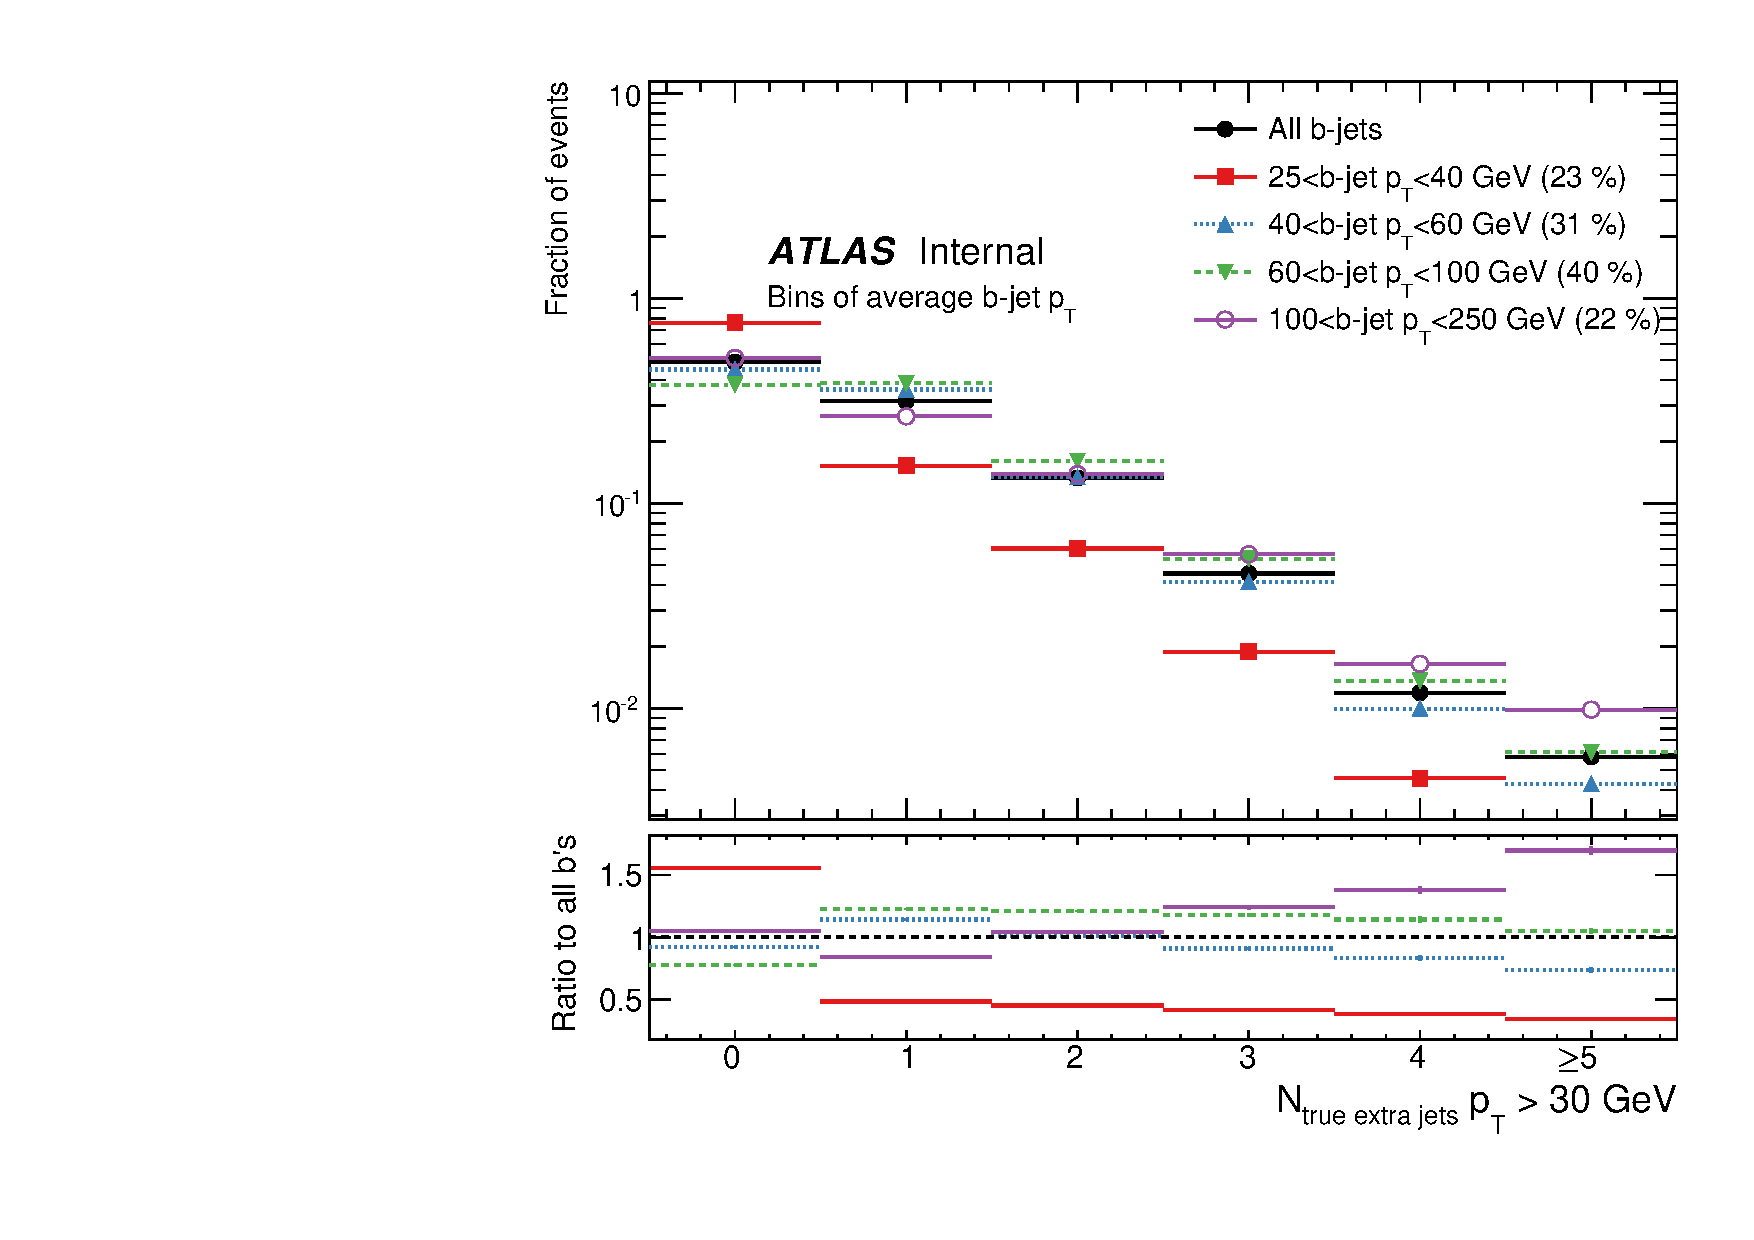
\includegraphics[width=0.45\textwidth]{fig/TruthNotReco/BJetNJets30.pdf}}
\subfloat{
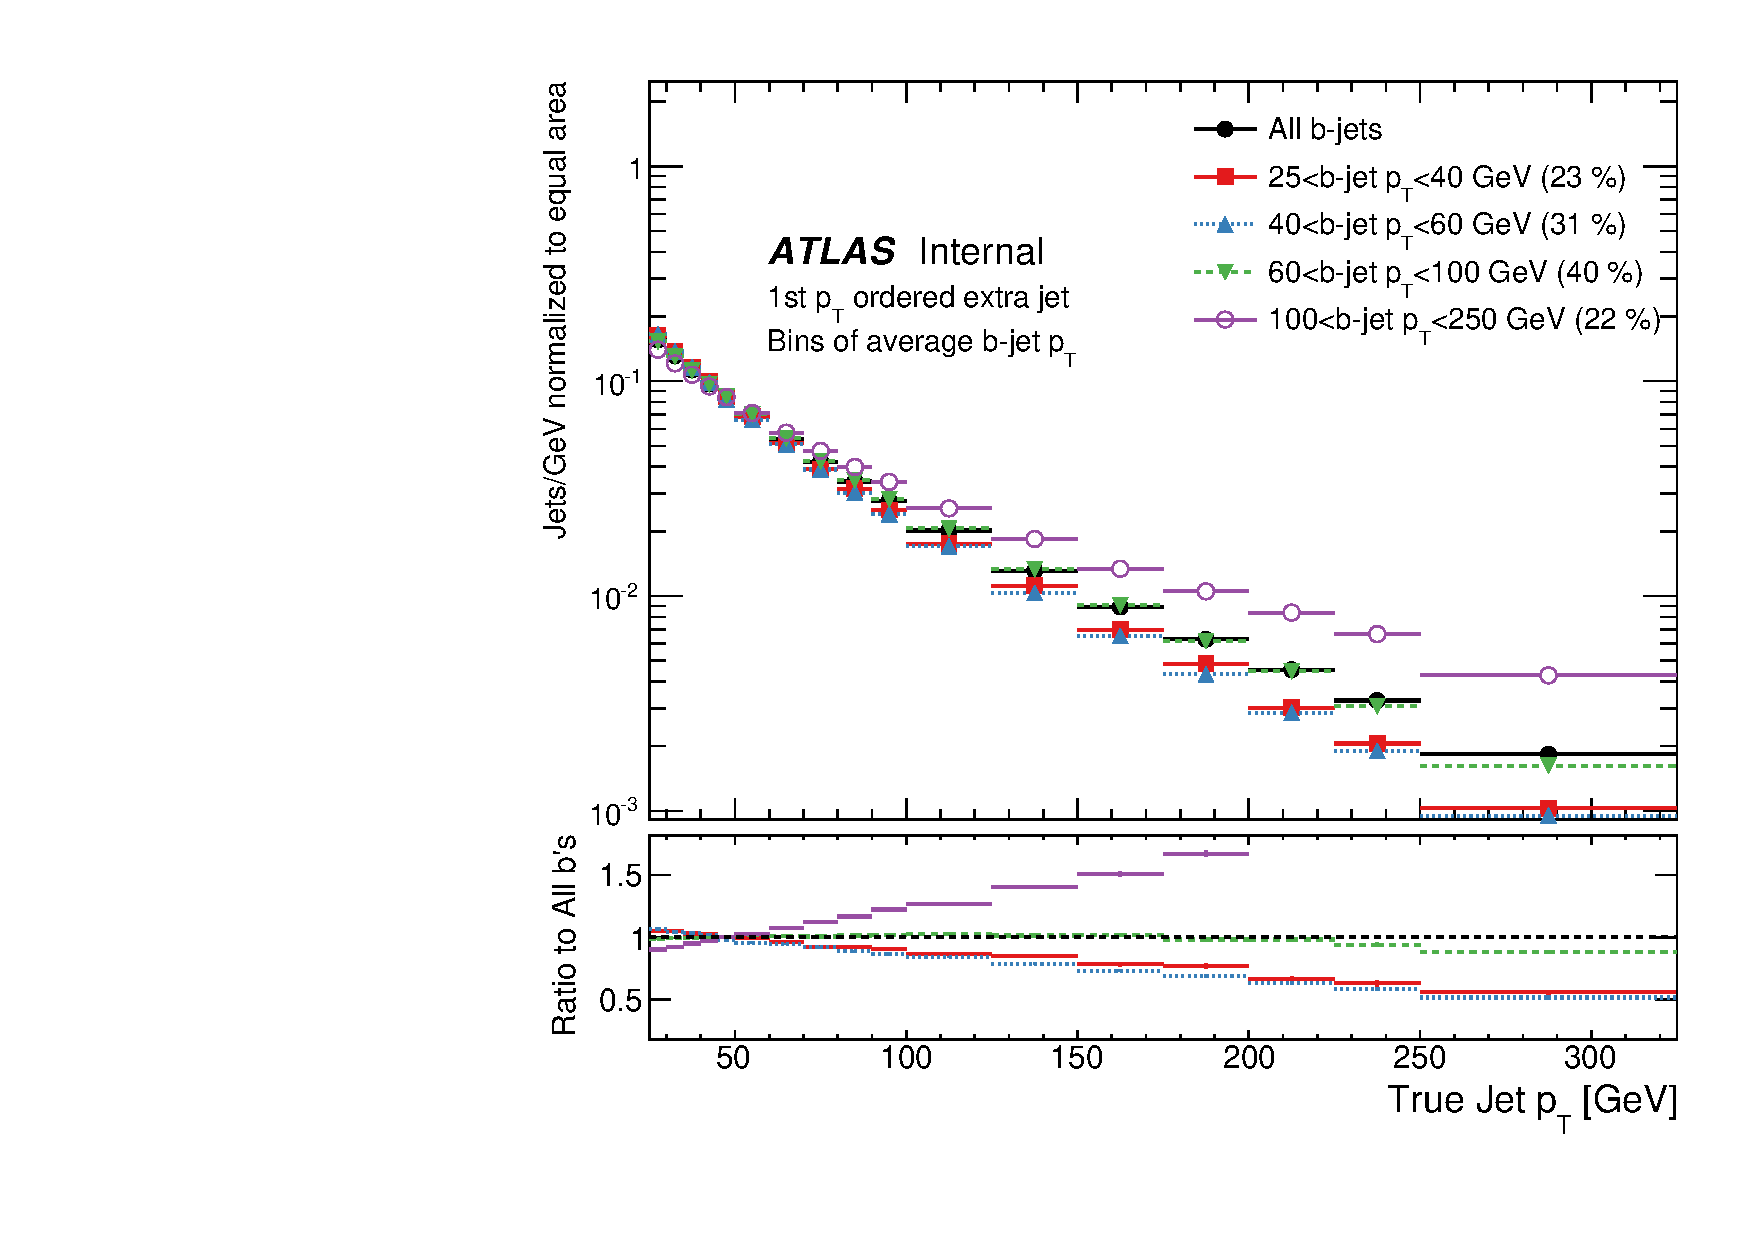
\includegraphics[width=0.45\textwidth]{fig/TruthNotReco/BJetPtJet0.pdf}}
\\
\subfloat{
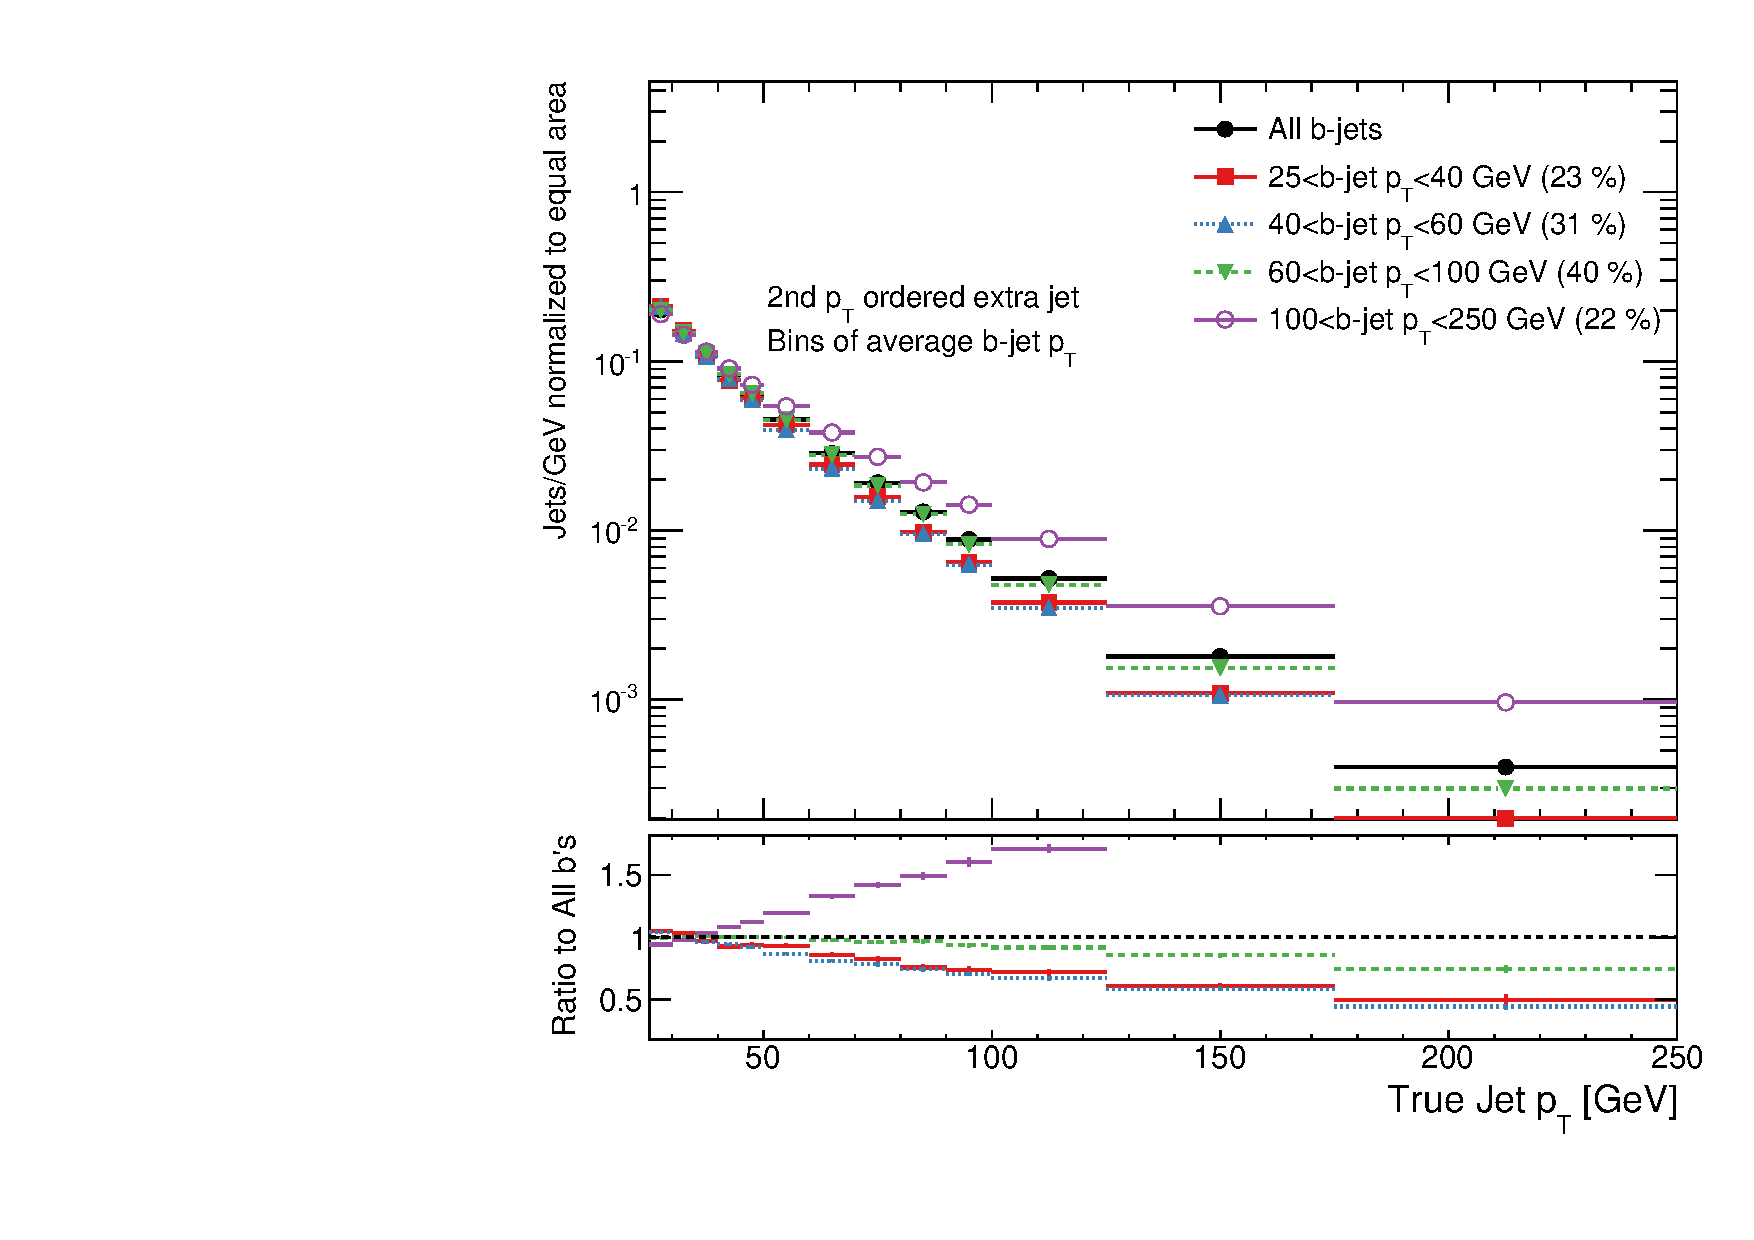
\includegraphics[width=0.45\textwidth]{fig/TruthNotReco/BJetPtJet1.pdf}}
\subfloat{
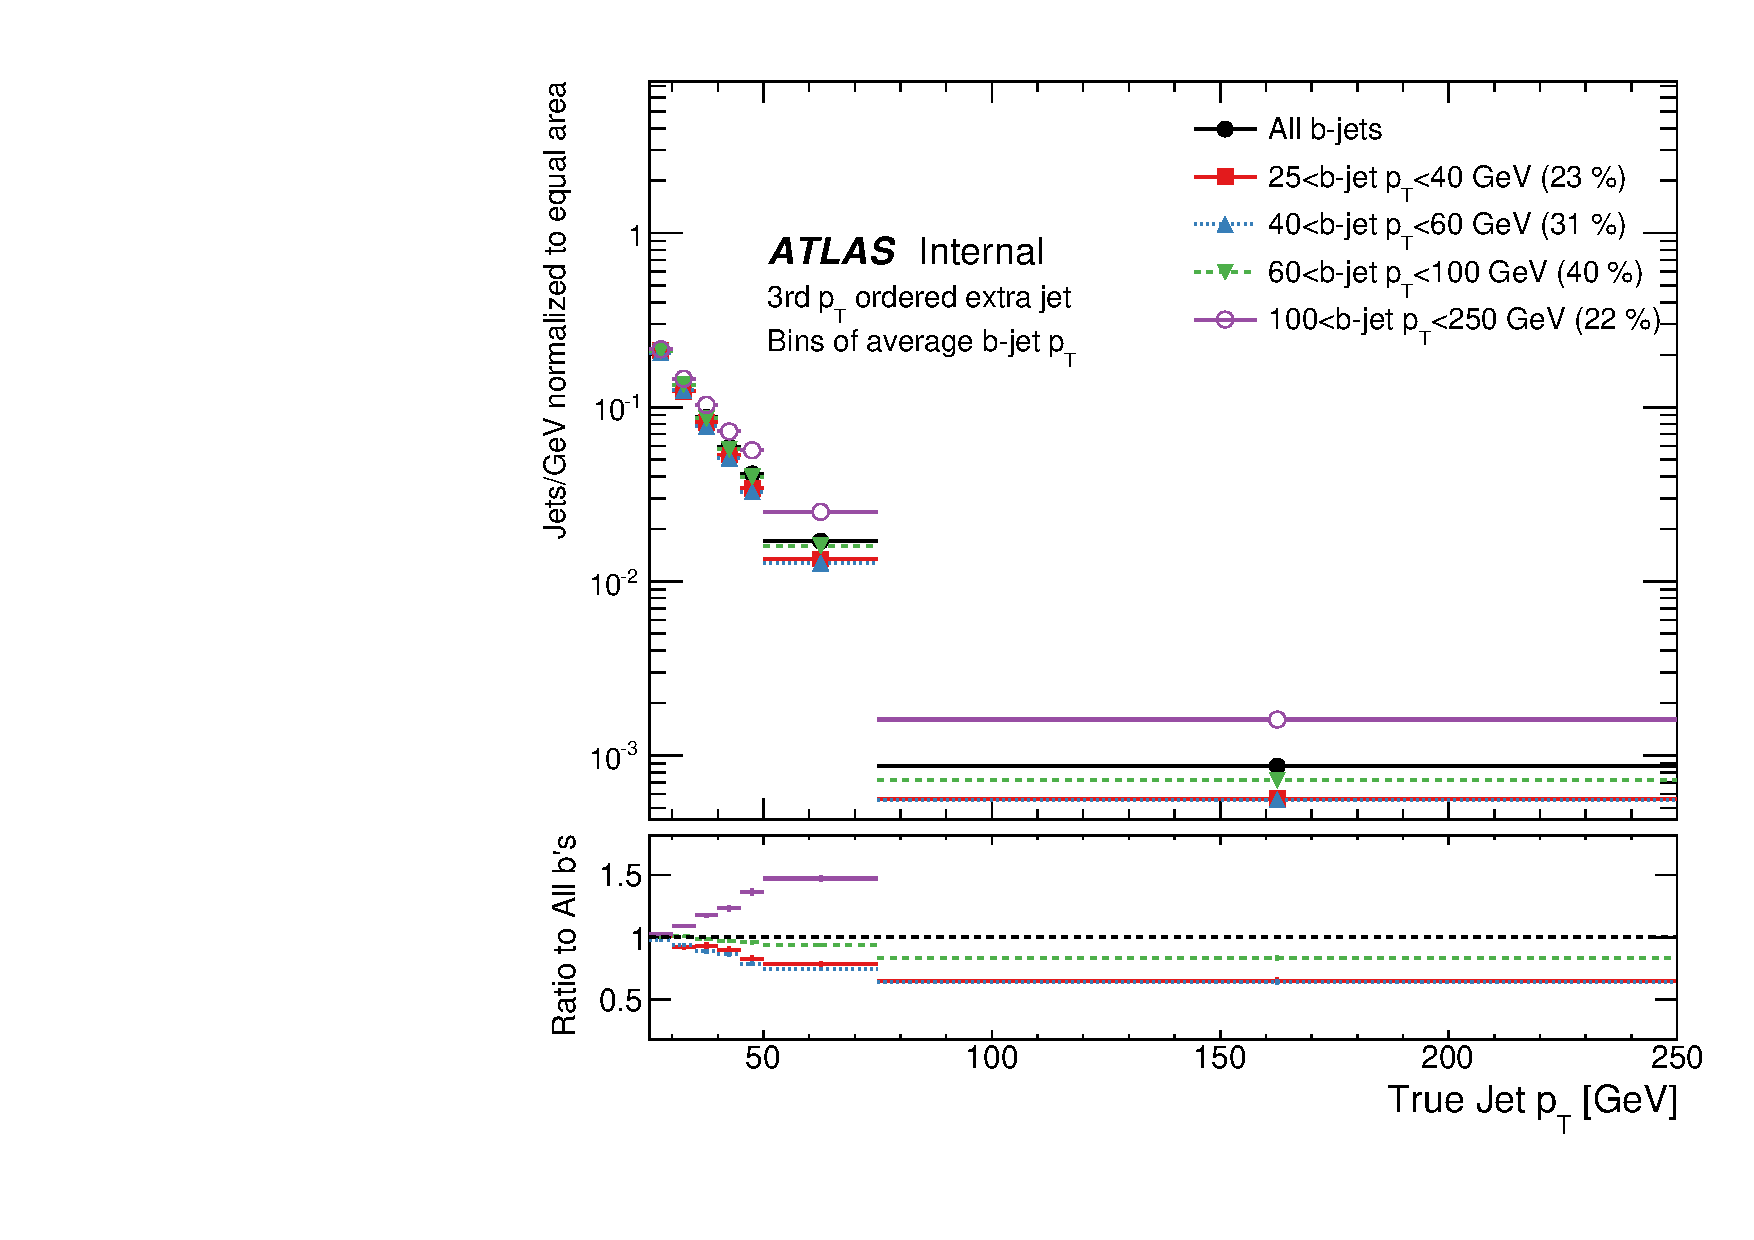
\includegraphics[width=0.45\textwidth]{fig/TruthNotReco/BJetPtJet2.pdf}}
\caption{Distributions of the truth (a) extra jet multiplicity, (b) leading extra jet \pt, (c) subleading extra jet \pt and (d) subsubleading extra jet \pt in bins of the average of the \pt of the two truth $b$-jets used to select the event. Each distribution is normalized by 
the number of events falling in that bin. Events were simulated with \powpy~\ttbar and required to pass the fiducial truth $e\mu$+2 $b$-jet selection.}
\label{fig:bjetdep}
\end{figure}


\subsubsection{Event selection correction factors}
\label{ss:unfcorr}

To correct for the effects discussed above, bin-by-bin correction factors $f^i$ are applied to the 
unfolded distribution as shown in Equation~\ref{eqn:unffinal}. These factors are derived by 
comparing unfolded simulated events that pass the reconstruction selection (with no particle level event selection) to
particle level truth distributions where no reconstruction requirements are applied.
Each bin's correction factor is given by:
\begin{equation}
f^i \equiv \frac{{\mathscr N}^i_{\textrm{true}}} {{\mathscr N}^i_{\textrm{unf}}}
\label{eqn:corrf}
\end{equation}
The simulated data used for this study includes \ttbar\ and single top events with their relative contributions determined
from their NLO cross sections. ${\mathscr N}^i_{\textrm{true}}$ and ${\mathscr N}^i_{\textrm{unf}}$ are normalized by number of events passing \emubb\ selection at the reconstructed and particle level, respectively. Since the final measurement given by Equation~\ref{eqn:unffinal} is normalized by the number of events in data, the correction factor $f^i$ corrects only for the bias in the extra jet spectrum, not the efficiency in number of events.
Figure~\ref{fig:bincorr} shows the correction factors obtained using different choices of generator for the \ttbar\ component.
The final correction factors used for data are taken from the baseline \powpy\ sample. Systematic uncertainties associated with generator dependence of this factor are discussed in Section~\ref{ss:unfsystt}.


% with the average difference 
%between \powpy\ and the other two generators as the systematic uncertainty. 
%The values of the correction factors are presented in Table~\ref{t:tcorr} in Appendix~\ref{app:tcorr}.



\begin{center}
\begin{figure}
\subfloat{
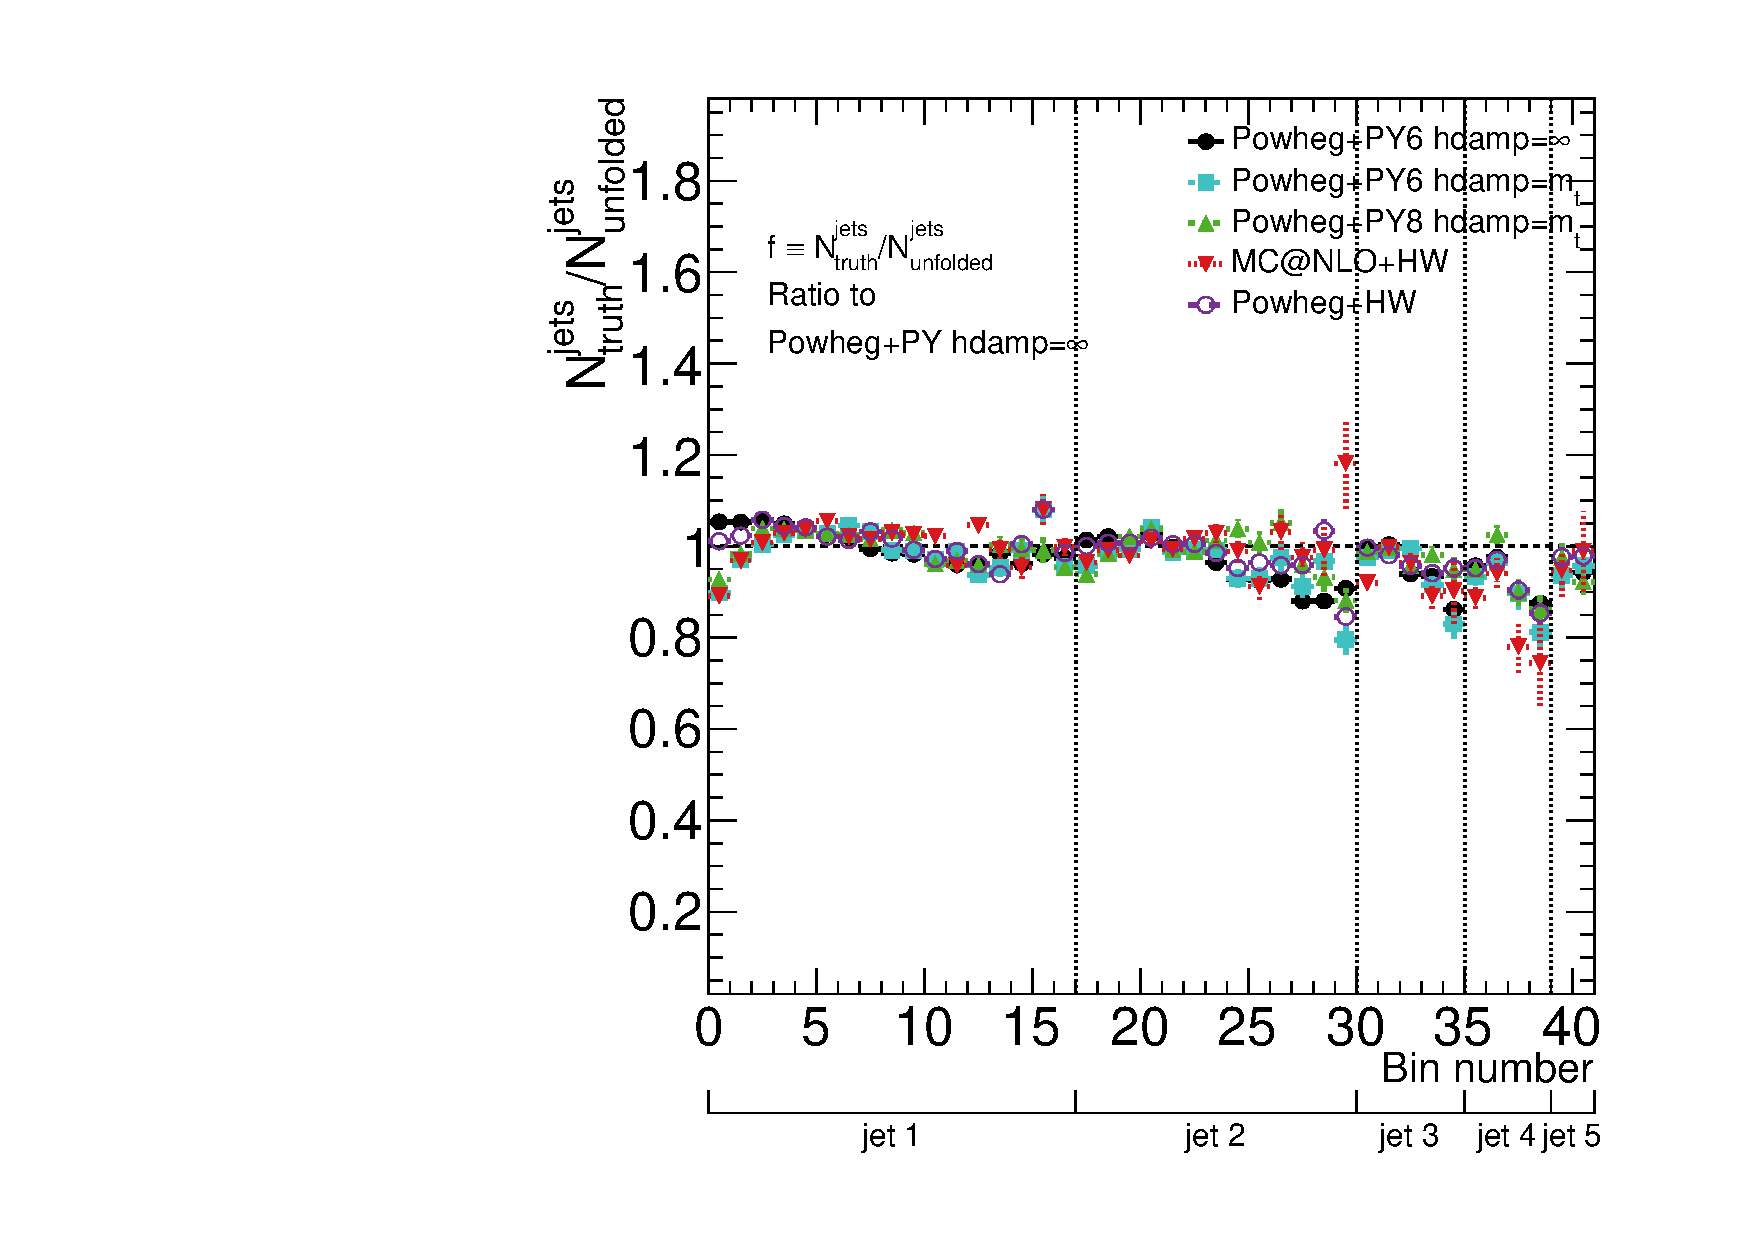
\includegraphics[width=0.45\textwidth]{fig/Unfolding/CorrFactors.pdf}}
~
\subfloat{
 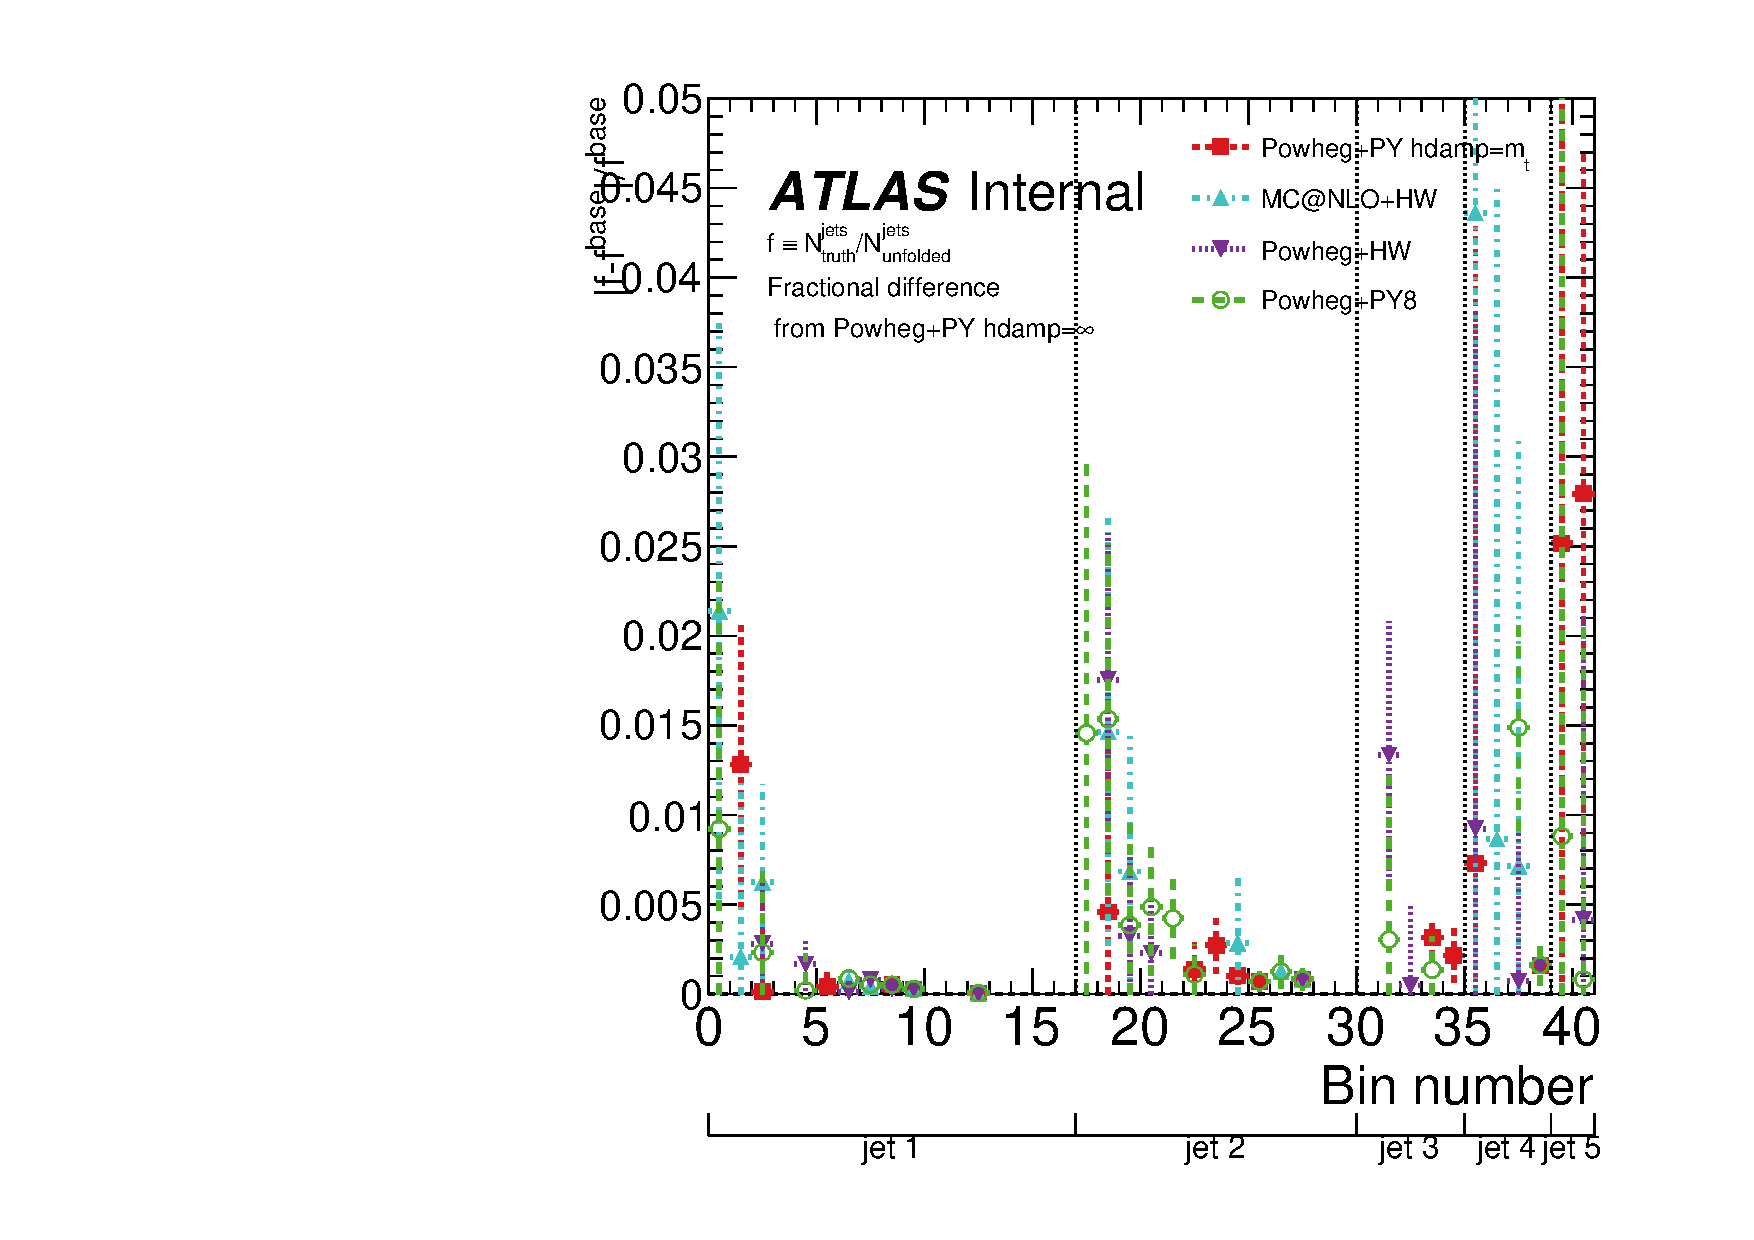
\includegraphics[width=0.45\textwidth]{fig/Unfolding/FractionCorrectionDiff.pdf}}
\caption{(a) Ratio of unfolded extra jets to truth extra jets different \ttbar generators (including a 2.9\% contribution from single top). (b) Fractional difference of the correction factorfrom baseline for different generators. Extra jets in events passing reconstructed and truth selection for each generator are added to single top and used to fill a response matrix. Then each generator is unfolded against itself, using all selected reconstructed events. Extra jet truth distributions are made without any reconstruction requirements. Finally, the unfolded distribution is divided by the truth distribution to obtain a correction factor for each bin.
\label{fig:bincorr}}
\end{figure}
\end{center}




\section{Validation}
%%COVARIANCE DISCUSSION HERE

\texttt{ RooUnfold} allows propagation of the full covariance matrix of the measured distribution through the unfolding. 
The package returns a covariance matrix, which is used to determine the uncertainties
on the unfolded spectrum. %and an inverse covariance matrix, which is used to calculated the $\chi^2$ betweenthe unfolded data and a predicted truth spectrum including correlations.
The covariance matrix $X$ on the unfolded distribution is calculated via pseudoexperiments. The diagonal elements of this covariance matrix give the uncertainties on the bins of \pt\ and rank. 

% The inverse of the covariance matrix is needed to compute the \chisq\ agreement between the unfolded and truth distributions. However, the regularized covariance matrix $X^{\tau}$ is singular and cannot be inverted. 
% Therefore, using and appropriate change of variable, the non-regularized inverse covariance matrix from the unfolding 
% ($X^{-1}$) can be used to compare true and unfolded distributions (see Eq. 53 in Ref.~\cite{svd}). This subtle distinction is discussed in more explicit detail in Ref.~\cite{svdphystat}.

The agreement between an unfolded spectrum and truth distribution can be estimated using a $\chi^2$ test (including correlations among bins):
\begin{equation}
\chi^2= \left( {\mathscr N}_{\textrm {unf}}- {\mathscr N}_{\textrm {true}} \right)^{T} X^{-1}\left( {\mathscr N}_{\textrm {unf}}- {\mathscr N}_{\textrm {true}} \right)
\label{eq:unfchi2}
\end{equation}
 The inverse covariance matrix, $X^{-1}$, is determined using SVD with \texttt{ SciPy}~\cite{scipy}.

This \chisq\ is used validate the unfolding procedure with different MC generators in Sections~\ref{ss:close}-\ref{ss:stress}, as well as to assess the agreement of generators with the fully corrected data in Section~\ref{sec:results}.
\subsection{Closure test}
\label{ss:close}
The closure test validates the unfolding procedure using simulation. The stability of unfolding can depend on the statistical power of the input data. To ensure that the the closure test appropriately accounts for this effect, the test is performed using pseudoexperiments with the same statistical power as the data.

In the closure test, the baseline \ttbar+3\% $Wt$ simulation is used to fill the migration matrix and
one thousand pseudoexperiments are performed using randomly chosen subsamples of events.  Each pseudoexperiment is chosen
so the number of events is equal to that of data. 
The extra jet distribution from each pseudoexperiment is then unfolded.  Each unfolded distribution is 
compared to the truth distribution obtained from the full sample of events used to train the migration matrix. 

The bias $B^i={\mathscr N}^i_{\textrm{ truth}}-{\mathscr N}^i_{\textrm{unfold}}$ and 
pull $P^i=({\mathscr N}^i_{\textrm{truth}}-{\mathscr N}^i_{\textrm{unfold}})/\sigma_{\textrm {unfold}}$ 
distributions are measured for each bin $i$. 
Figure~\ref{fig:UnfoldPull} shows the mean pull and its uncertainty in bins of \pT\ for jets of rank~1 through~5.  The shaded bands indicate
the width of the pull distribution, obtained from a Gaussian fit.
The pull distributions for each bin are shown in Appendix~\ref{app:unfoldpull}. 
The mean pull is close to zero and has a width close to unity.  This demonstrates that the unfolding procedure has no 
significant bias and that the statistical uncertaintainties on the unfolded distribution are properly estimated. Additional test of the unfolding are provided in Appendix~\ref{app:unfoldval}. 

In addition to the pull and bias, the average \chisq\ between the unfolded pseudoexperiments and the true distribution is computed using Equation~\ref{eq:unfchi2}.  The \chisq\ obtained in the closure test is 42 for 41 degrees, indicating that the
inverse covariance matrix returned from RooUnfold appropriately estimates the correlated uncertainties. 

\subsection{Stress test}
\label{ss:stress}
`Stress' tests assess the effect of the input \pt\ spectrum on the unfolding algorithm by unfolding pseudoexperiments produced from alternate \ttbar\~MC generators (described in Section ~\ref{sec:samples}) using the response matrix and correction factors
obtained from the baseline. 

To study the stability of the unfolding with respect to changes in the input jet \pt\ and multiplicity spectra, pseudoexperiments are constructed by reweighting the truth jet spectrum in the baseline MC sample. The weight for each bin is given by the ratio of the alternative generator to the baseline\footnote{An alternative reweighting procedure where the ratios were fit to a smooth function was also studied. Changes with respect to the procedure described here were small}. This procedure isolates the uncertainty associated with the choice of spectrum from other sources of instability (e.g. JES), which are accounted for separately. %ADD MORE EXPLANATION??

Stress tests have been performed using the following samples: \pow+\py, \pow+\hw, \madpy, \mcnlohw, \peight, \hdamp, RadHi \madpy\ and RadLo \madpy. Each of the alternate \ttbar\ samples are unfolded with 1000 pseudoexperiments against a migration matrix filled from the baseline \ttbar\ simulation. In both the migration matrix and the samples, a 3\% constribution from single top is included. Correction factors ($f$ and $g$ in Equation~\ref{eqn:unffinal}) are also taken from the baseline.

The pull distributions for the alternate generators unfolded against the baseline are provided in Appendix~\ref{app:stressiter}, including studies of number of iterations.

Figure~\ref{fig:fracbias} shows the fractional bias obtained for the stress test for four representative alternative generators. Though bin-to-bin fluctuations around zero are visible, these fluctuations fall largely within the one sigma error contour. For \mcnlohw, the disagreements become large for jets of rank 3 and higher. The jet multiplicity in \mcnlohw\ at reconstruction level is signifigantly lower than the data. For \madpy\ deviations above the one sigma level are observed for low jet \pt. The \madpy\ is signifigantly steeper than that of \powpy. This will affect the size of the feed-in correction $g_i$. The differences with respect to \madpy\ are included in the systematic uncertainties described in Section~\ref{ss:unfsystt}.

\begin{figure}
\subfloat{
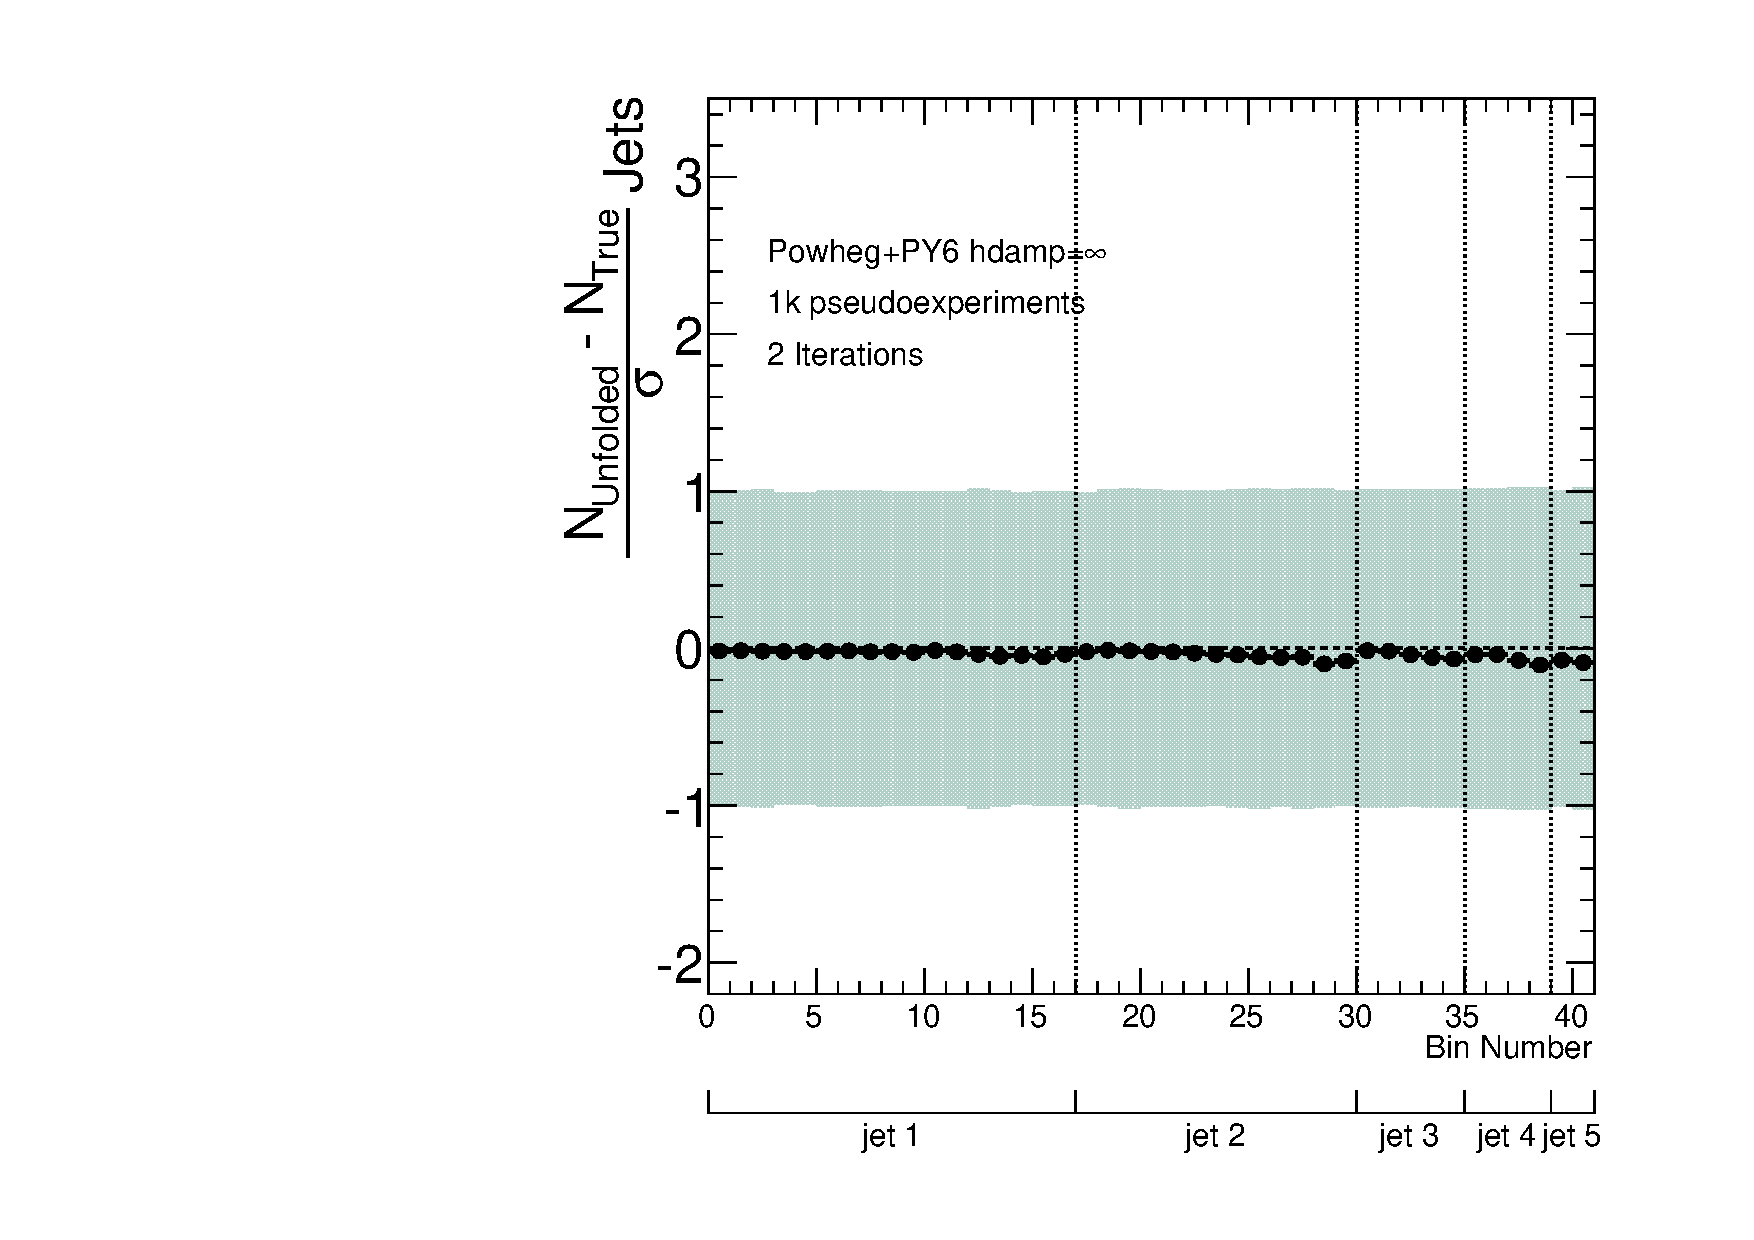
\includegraphics[width=0.45\textwidth]{fig/Stress/117050atlfast/Pull2Iterations.pdf}}
~
\subfloat{
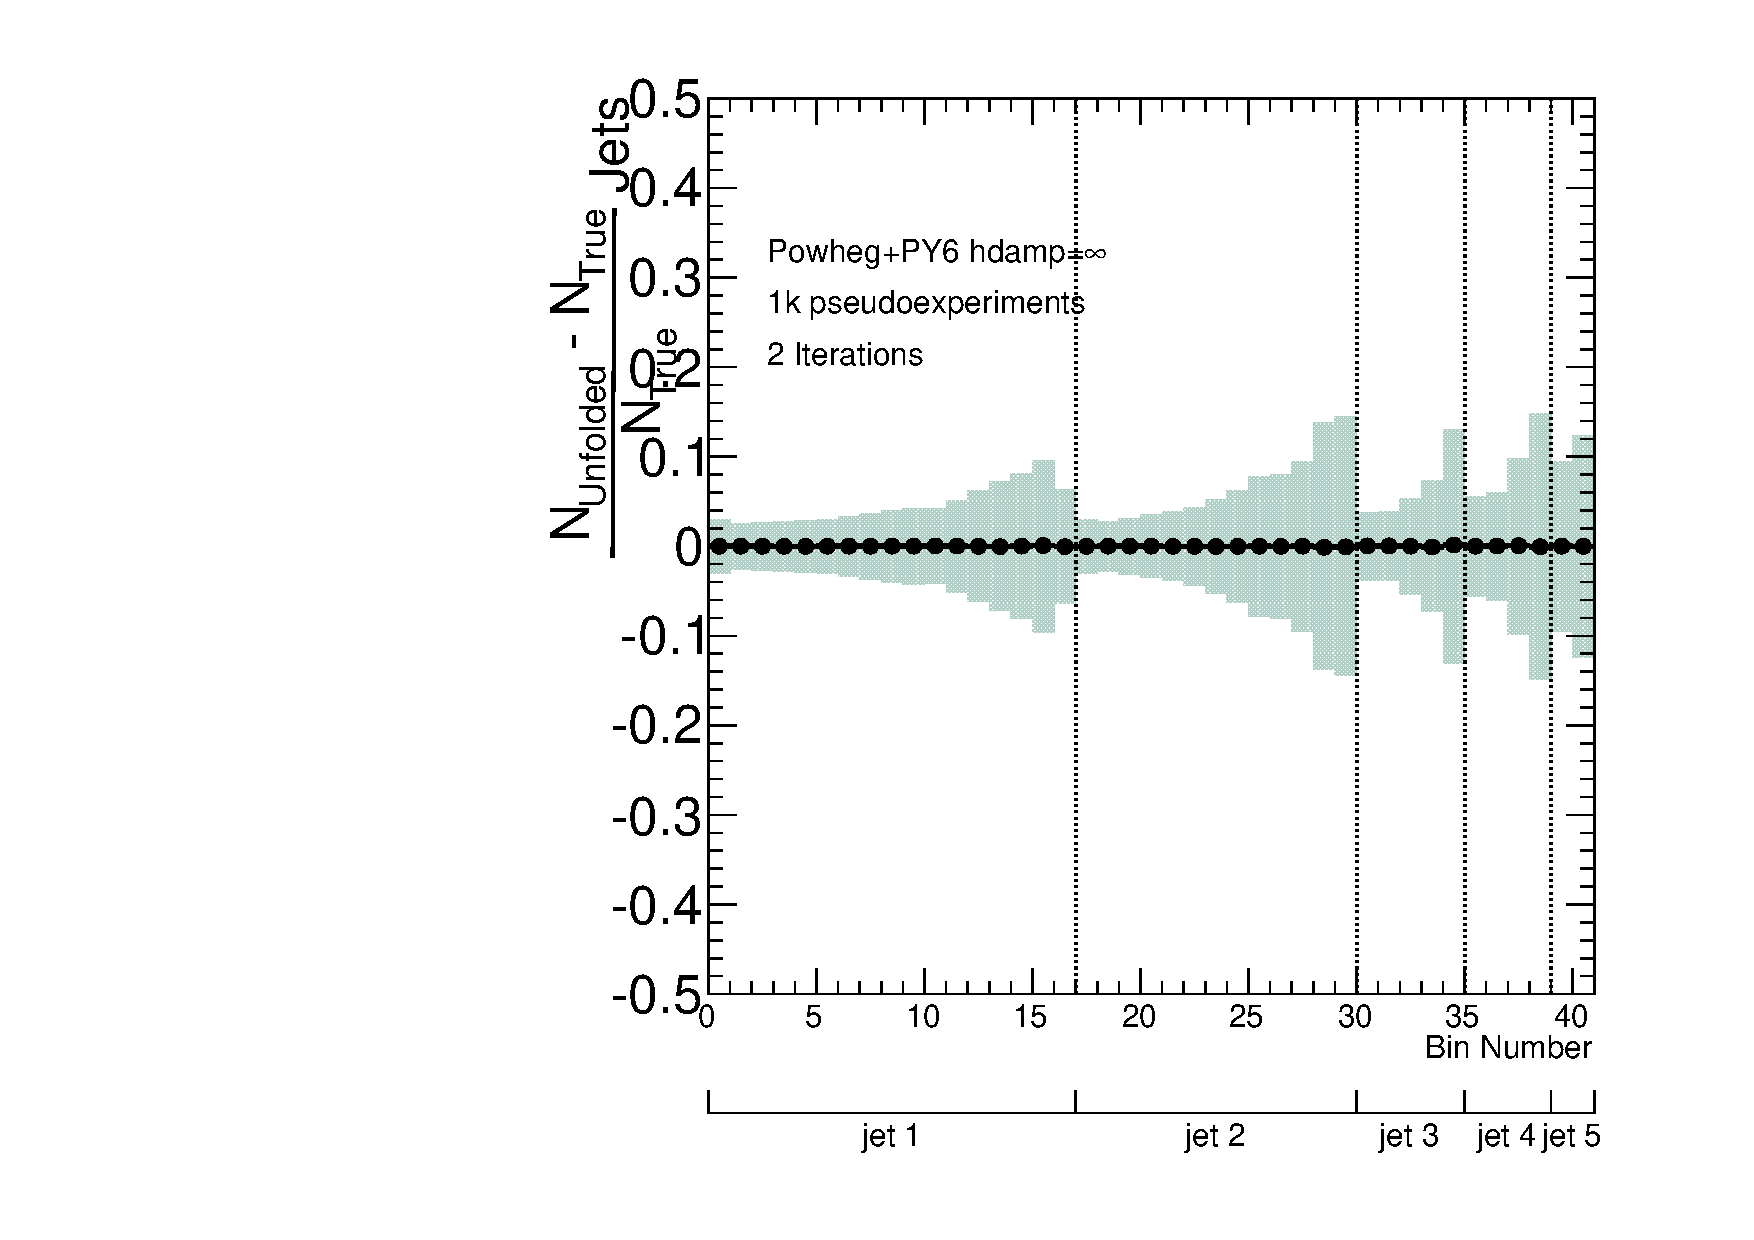
\includegraphics[width=0.45\textwidth]{fig/Stress/117050atlfast/FracBias2Iterations.pdf}}
\caption{(a) Pull distribution and (b) fractional bias for the extra jets from the baseline \ttbar simulation unfolded against a matrix filled with the baseline \ttbar simulation with all correction factors. The Bayesian unfolding method with 2 iterations is used. One thousand pseudoexperiments, each the size of the events in data, are randomly selected from the sample and unfolded. Each bin of the pull distribution over the pseudoexperiments is fit with a gaussian. The black points show the fitted mean of each bin. A fitted mean of zero shows the unfolding is not signifigantly biased. The blue band shows the fitted $\sigma$ of each bin. A fitted $\sigma$ of one shows the unfolding correctly estimates the errors.}
\label{fig:UnfoldPull}
\end{figure}

\begin{figure}
\subfloat{
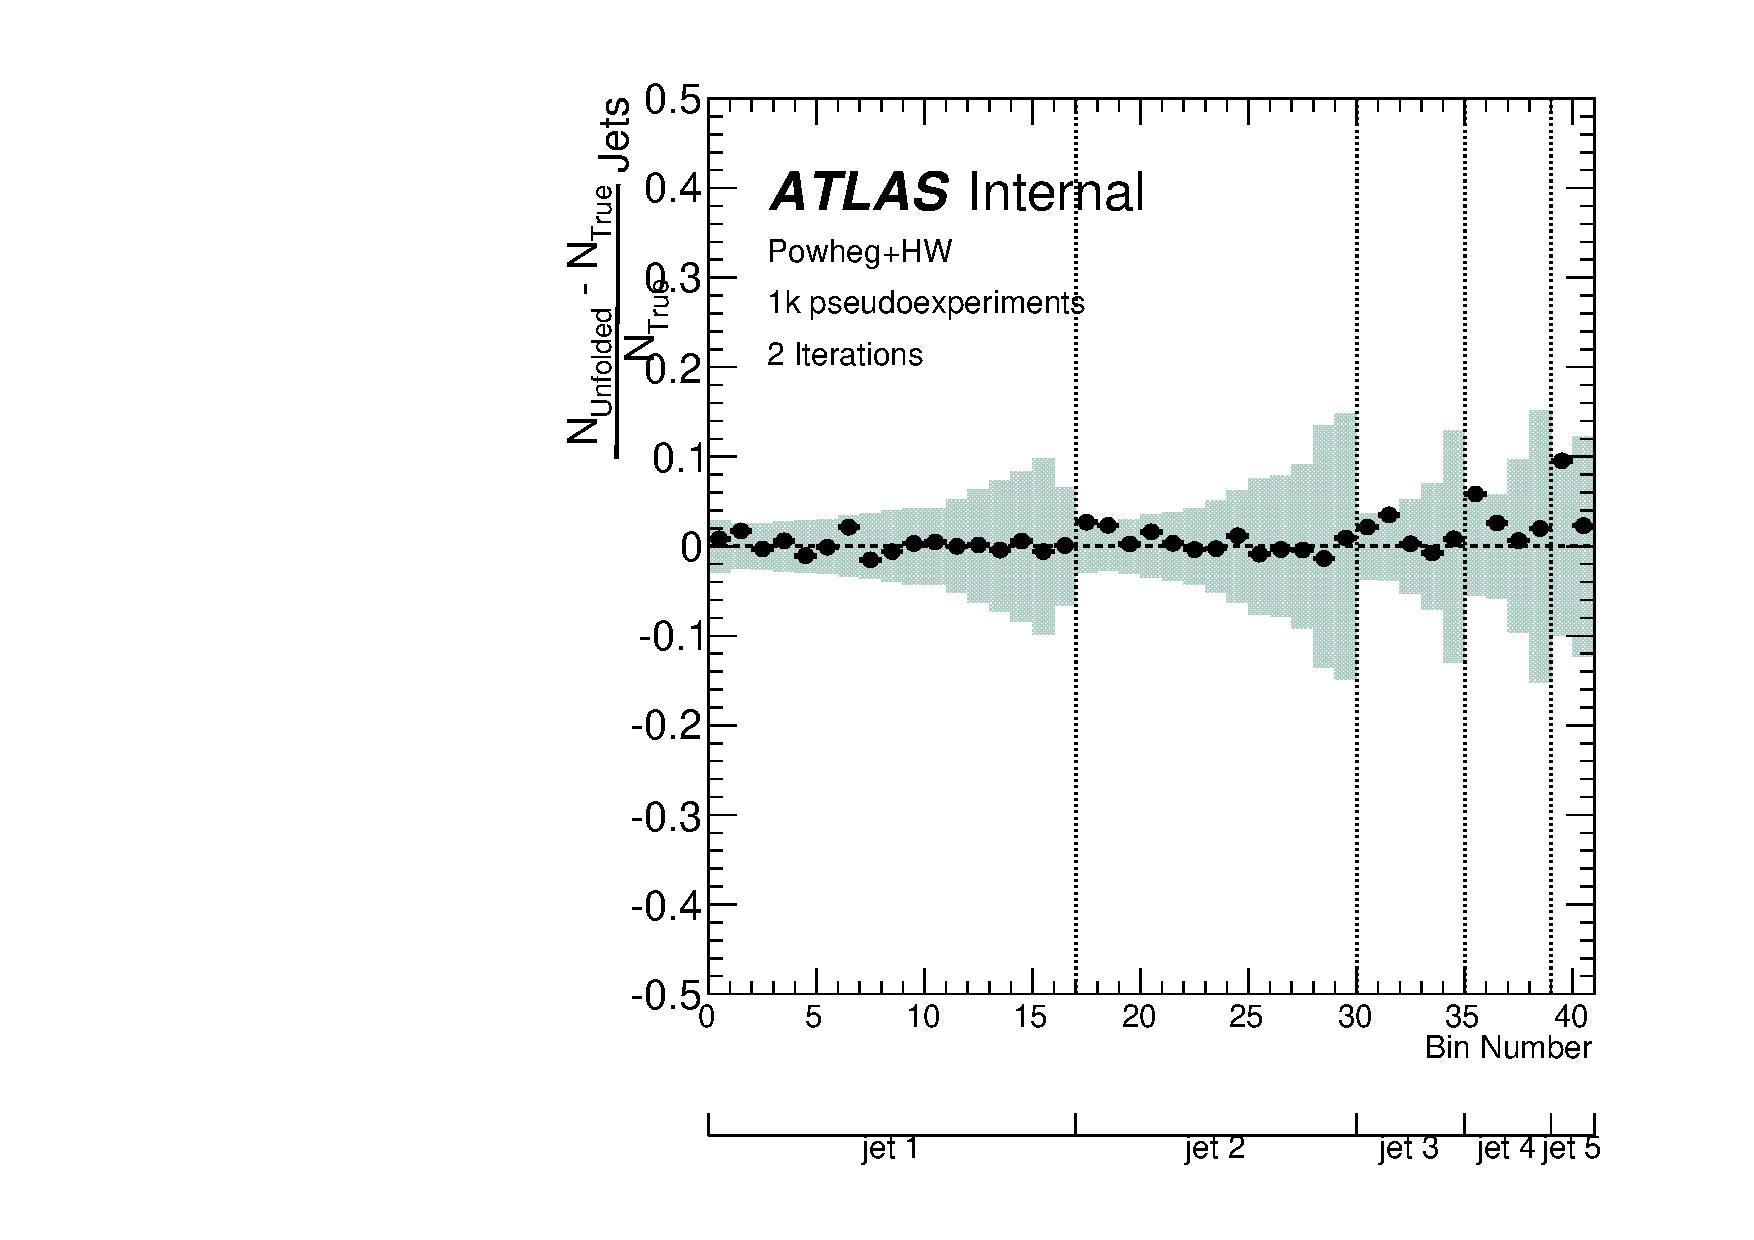
\includegraphics[width=0.45\textwidth]{fig/Stress/105860atlfast/FracBias2Iterations.pdf}}
~
\subfloat{
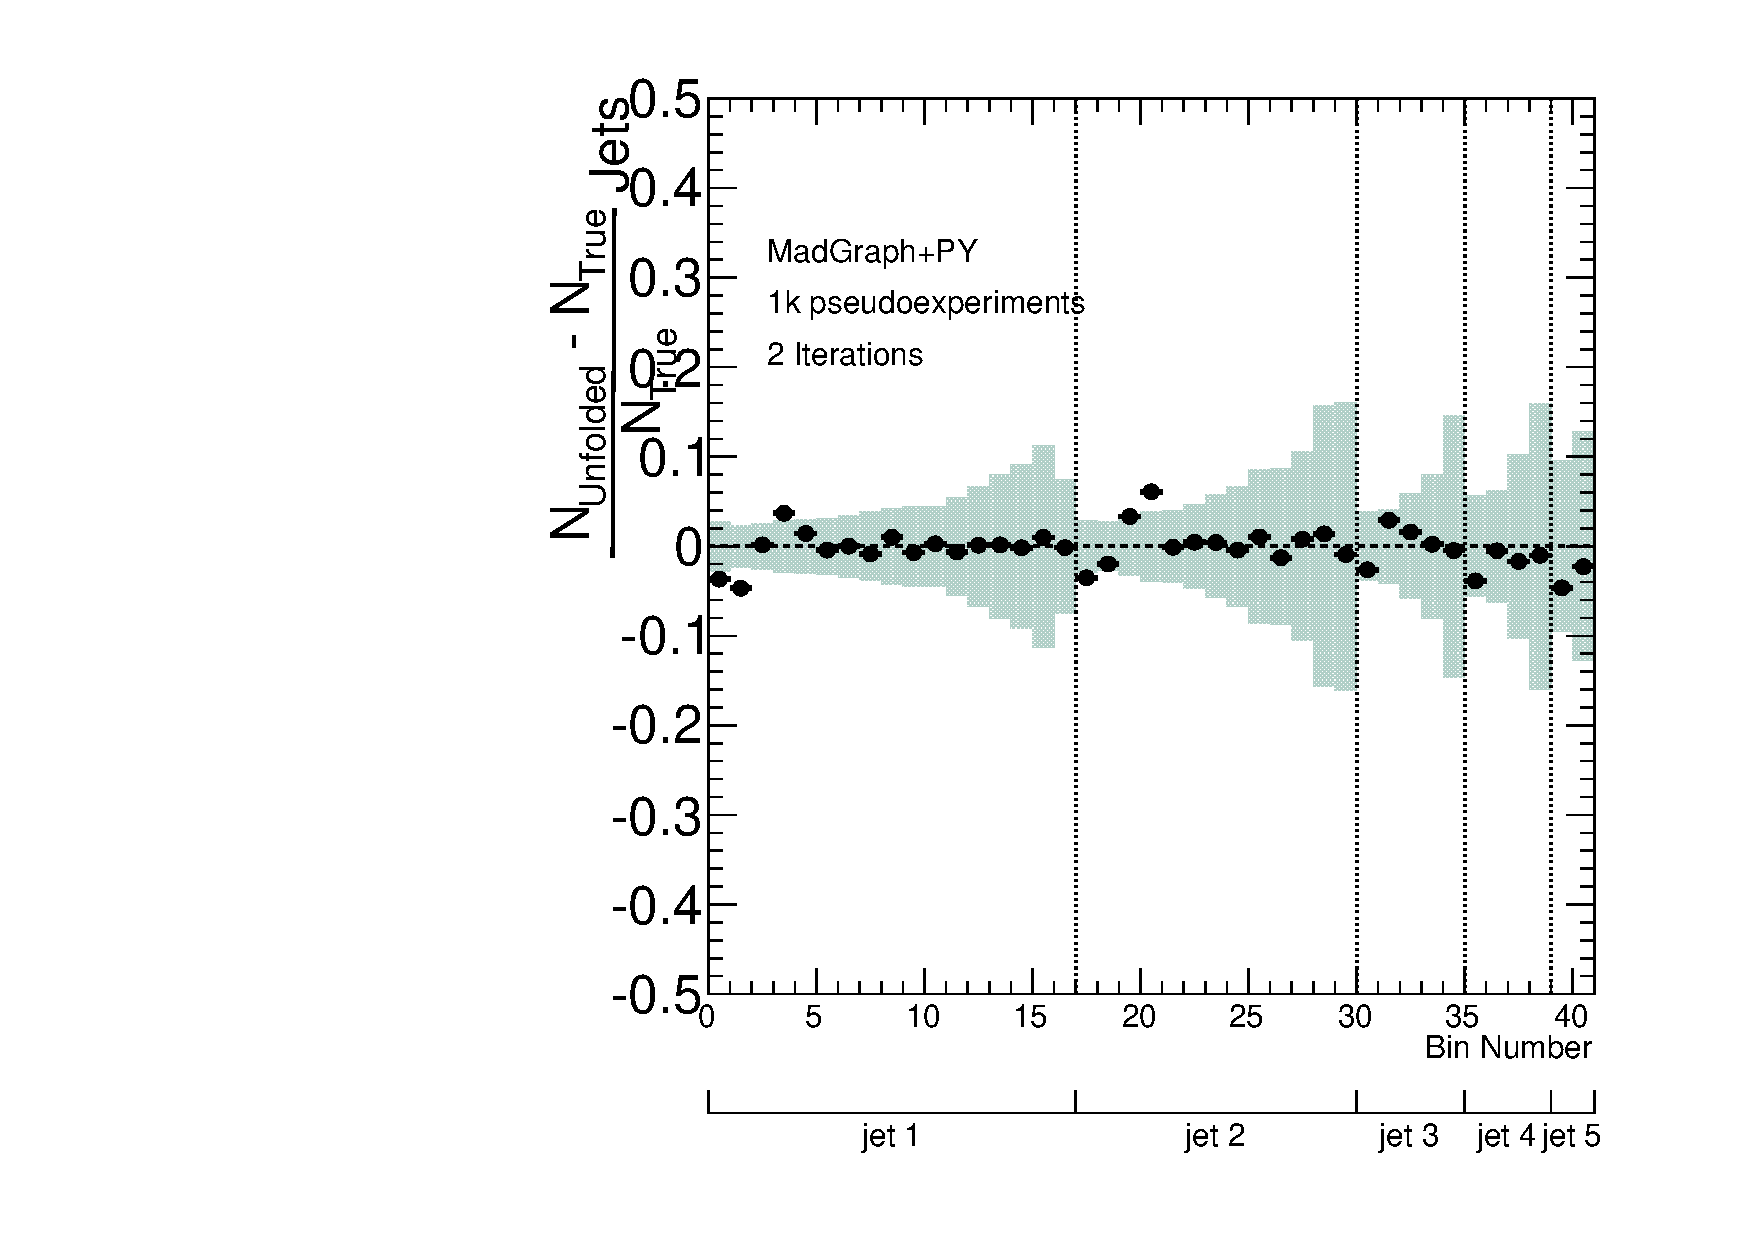
\includegraphics[width=0.45\textwidth]{fig/Stress/110872atlfast/FracBias2Iterations.pdf}}
\\
\subfloat{
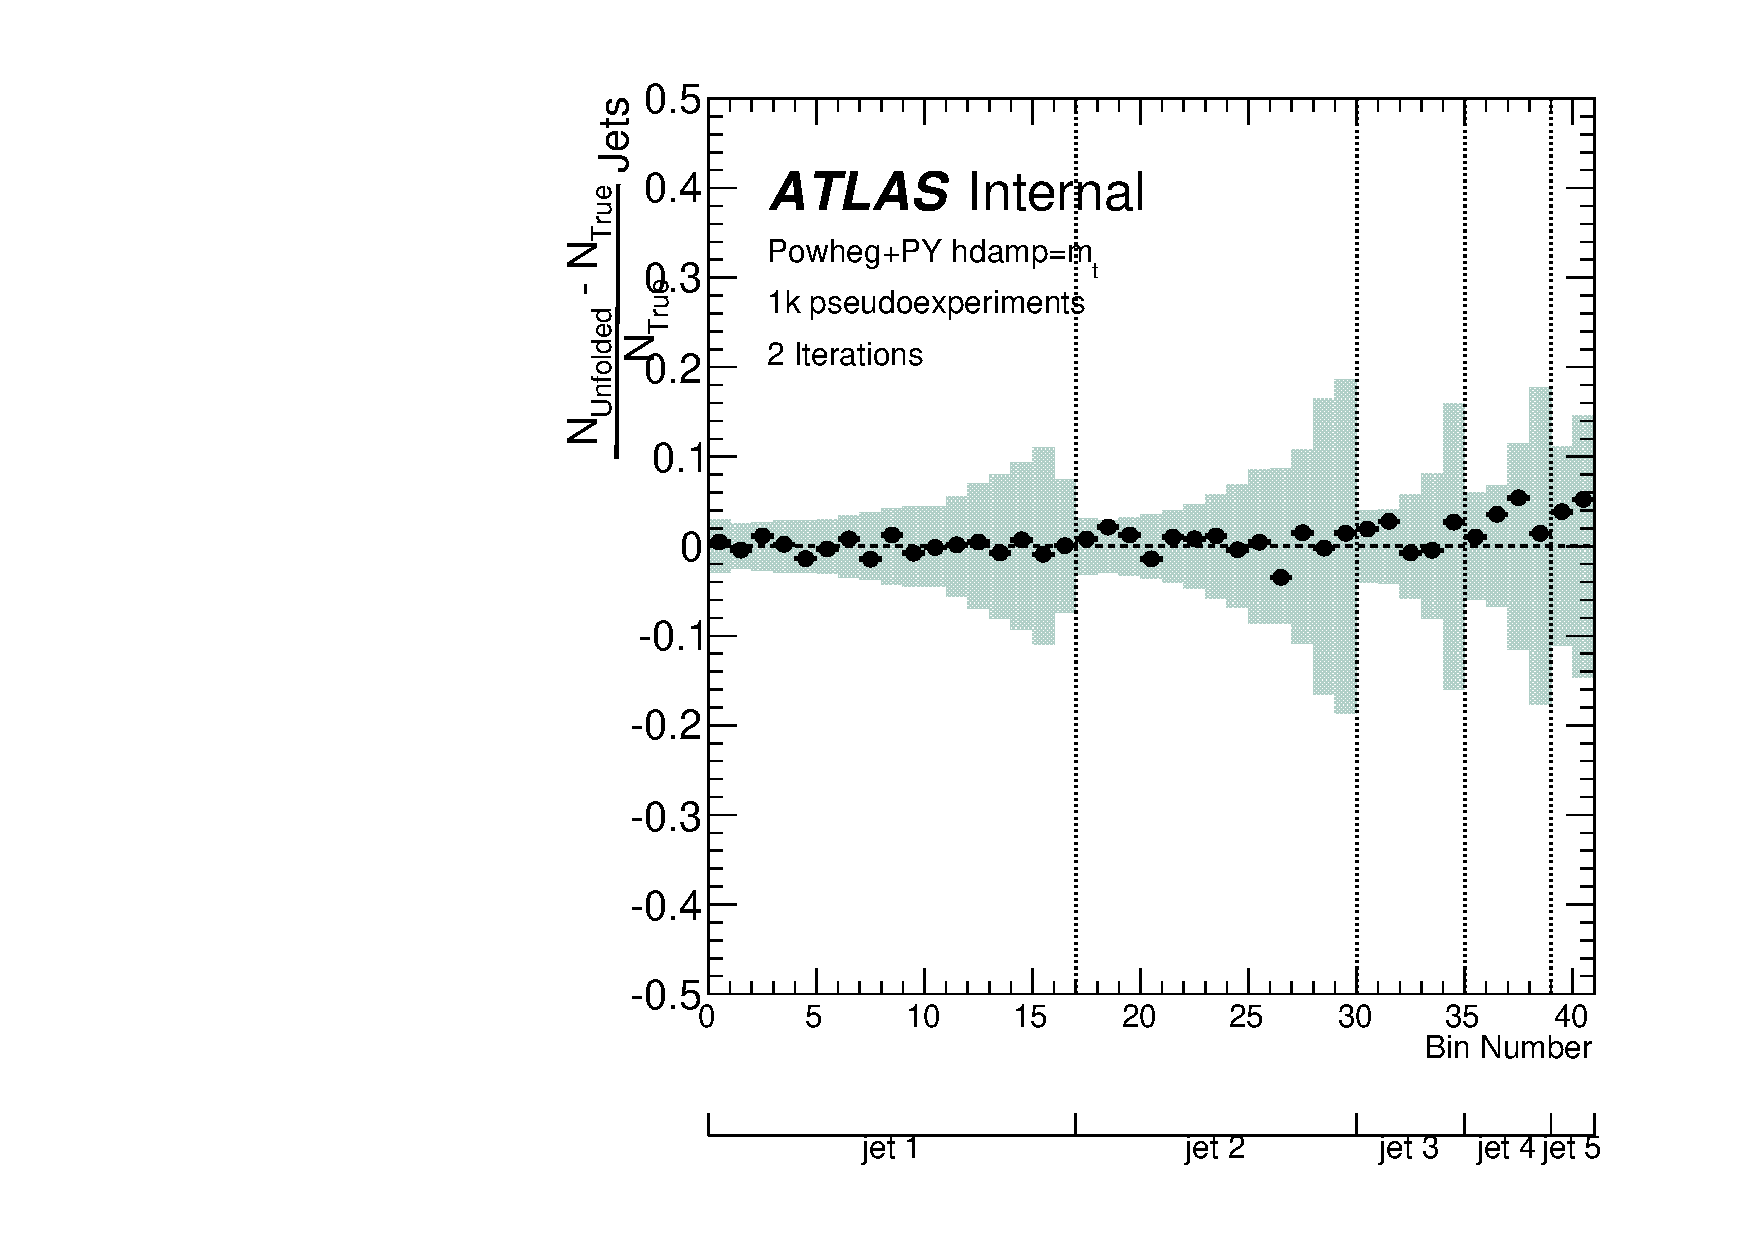
\includegraphics[width=0.45\textwidth]{fig/Stress/110404atlfast/FracBias2Iterations.pdf}}
~
\subfloat{
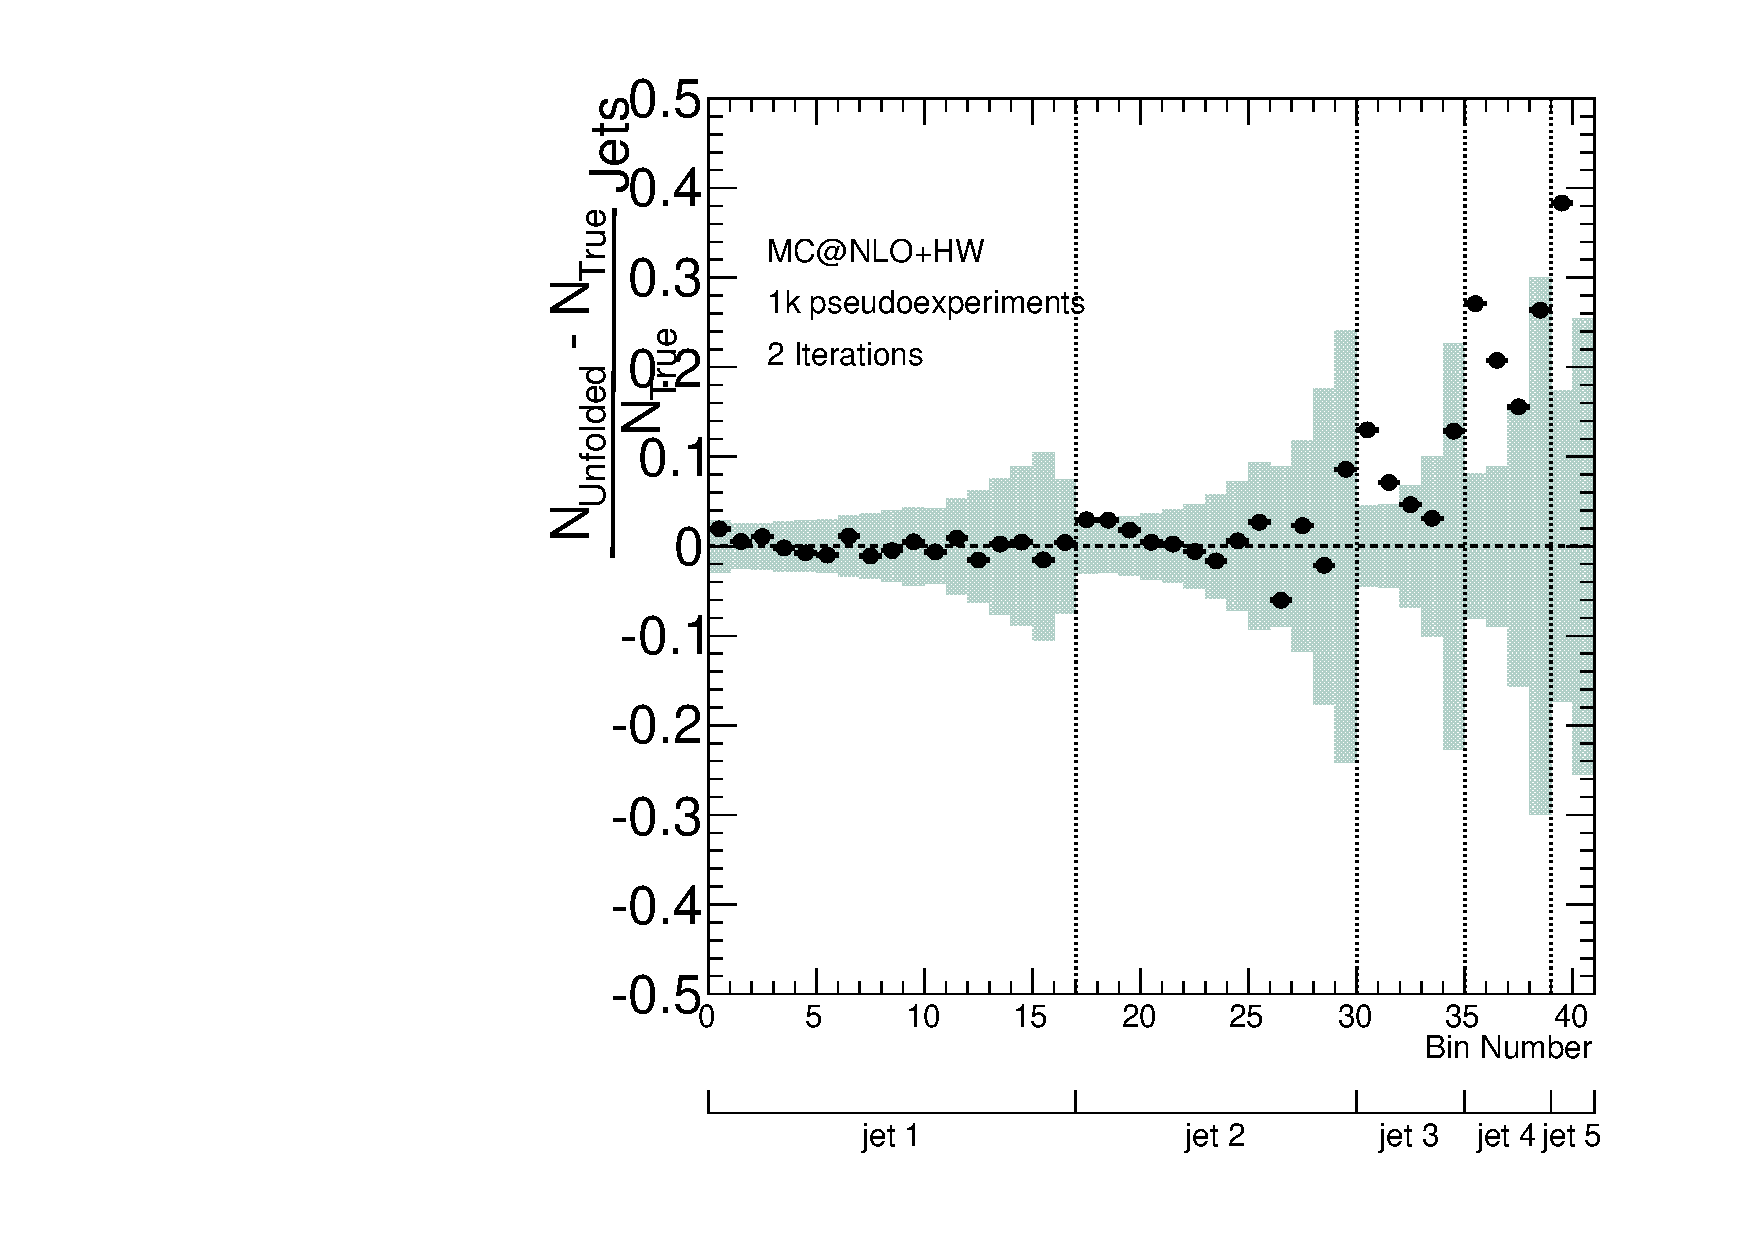
\includegraphics[width=0.45\textwidth]{fig/Stress/105200atlfast/FracBias2Iterations.pdf}}
~
\caption{Fractional bias distributions for pseudoexperiments from alternative generators unfolded against a matrix filled with the baseline simulation. The truth spectrum of the baseline sample is reweighted to match jet \pt\ and multiplicity spectra of (a) \pow+\hw (b) \madpy, (c) \hdamp, and (d) \mcnlohw~simulation. One thousand pseudoexperiments, each the size of the events in data, are constructed for each generator and unfolded. The Bayesian unfolding method with 2 iterations is used. Each bin of the distribution over the pseudoexperiments is fit with a gaussian. The black points show the fitted mean of each bin and the blue band shows the fitted sigma.}
\label{fig:fracbias}
\end{figure}
